\documentclass{article}

\usepackage[preprint]{neurips_2026}

\usepackage[utf8]{inputenc}
\usepackage[T1]{fontenc}
\usepackage{amsmath,amssymb,amsfonts}
\usepackage{amsthm}
\usepackage{url}
\usepackage{booktabs}
\usepackage{graphicx}
\usepackage{algorithm}
\usepackage{algpseudocode}
\usepackage{nicefrac}
\usepackage{microtype}
\usepackage{xcolor}
\usepackage{listings}
\usepackage[font=small]{caption}
\usepackage{wrapfig}
\usepackage{hyperref}

\newtheorem{theorem}{Theorem}
\newtheorem{claim}{Claim}

% Python listings style for code snippets.
\lstset{
  basicstyle=\ttfamily\small,
  language=Python,
  numbers=none,
  showstringspaces=false,
  keywordstyle=\color{blue!55!black}\bfseries,
  commentstyle=\color{gray!60!black}\itshape,
  stringstyle=\color{green!45!black},
  frame=single,
  framerule=0.2pt,
  rulecolor=\color{gray!50},
  captionpos=b,
  xleftmargin=4pt,
  xrightmargin=0pt,
  breaklines=true,
  columns=fullflexible,
  aboveskip=4pt,
  belowskip=2pt,
}

% Give \thanks footnote marks real width so they don't overlap with the numeric
% affiliation superscript (style file sets them to zero-width by default).
\makeatletter
\renewcommand{\@makefnmark}{\hbox{$^{\@thefnmark}$}}
\makeatother


\makeatletter
\renewcommand{\@makefnmark}{\hbox{$^{\@thefnmark}$}}
\makeatother

\renewcommand{\thefootnote}{\fnsymbol{footnote}}
\setcounter{footnote}{1}

% \title{DualKV: Shared-Prompt Flash Attention for Efficient Policy Updates in Large-Rollout and Long-Context RL Training}
\title{DualKV: Shared-Prompt Flash Attention for Efficient RL Training with Large Rollouts and Long Contexts}
\author{
  Jiading Gai\textsuperscript{1,*} \quad
  Shuai Zhang\textsuperscript{1,*} \quad
  Xiang Song\textsuperscript{2}\thanks{Work done while at AWS.} \quad
  Bernie Wang\textsuperscript{1} \quad
  George Karypis\textsuperscript{3}\footnotemark[2]
  \\[4pt] 
  \textsuperscript{1}\textit{Amazon Web Services} \quad
  \textsuperscript{2}\textit{Google} \quad
\textsuperscript{3}\textit{University of Minnesota} \\
  \texttt{\{jiadingg, shuaizs, yuyawang\}@amazon.com} \quad \texttt{xiangsx@google.com} \quad \texttt{karypis@umn.edu} \\[2pt]
  \textsuperscript{*}\textit{Equal contribution.} \\[2pt]
  \textcolor{blue}{\url{https://github.com/amazon-science/dualkv-flash-attn-for-rl}}
}

\begin{document}
\maketitle

\begin{abstract}
Modern RL post-training methods such as GRPO and DAPO train on $N$ response sequences of $R$ tokens sampled from a shared prompt of $P$ tokens, but standard FlashAttention replicates all $P$ prompt tokens $N$ times across both forward and backward passes --- duplicating compute and memory on identical hidden states.
In large-rollout, long-context RL training ($N{\geq}16$, $P{\geq}8\text{K}$), this redundancy dominates the policy update cost.
We observe that in decoder-only models, causal masking makes prompt representations invariant across sequences at every layer, so all per-token operations (norms, projections, MLP) and attention can process the prompt once --- a property not yet exploited at the kernel level for training.
We propose \textbf{DualKV}, the first FlashAttention kernel variant that eliminates shared-prompt replication during RL training, via (1)~fused CUDA forward and backward kernels that iterate over two disjoint KV regions --- shared context and per-sequence response --- in a single kernel launch, and (2)~a data-pipeline redesign in veRL that repacks $N(P{+}R)$ tokens into $P{+}NR$ tokens per micro-batch, extending the token reduction from attention to the entire model by a factor $\rho = N(P{+}R)/(P{+}NR)$.
DualKV is mathematically equivalent to standard attention and introduces no approximation.
On Qwen3-8B GRPO training with 8$\times$H100 GPUs ($N{=}32$, 8K-context), DualKV achieves $1.63$--$2.09\times$ policy-update speedup, enables $2\times$ larger micro-batches, and raises MFU from $36\%$ to $76\%$. Similar gains hold for DAPO ($2.47\times$ speedup, $77\%$ MFU). At 30B MoE scale on 16$\times$H100, DualKV achieves $3.82\times$ policy-update and $3.38\times$ end-to-end step speedup over FlashAttention (which requires 4-way Ulysses sequence parallelism to avoid OOM).
\end{abstract}

%----------------------------------------------------------------------
\section{Introduction}
\label{sec:intro}
%----------------------------------------------------------------------

Modern RL post-training methods such as GRPO~\citep{shao2024deepseekmath} and DAPO~\citep{yu2025dapo} compute log-probabilities and gradients for $N$ response sequences that share a prompt of $P$ tokens. With standard FlashAttention-2 (FA2)~\citep{dao2023flashattention2}, the training micro-batch contains $N$ sequences of length $S_i = P + R_i$, repeating the $P$-token prompt $N$ times. Each forward and backward pass recomputes $K, V$ activations and their gradients over $(N{-}1) \times P$ redundant prompt tokens per layer.

Recent work demonstrates that model accuracy continues to improve with increasingly large rollout factors. \citet{lightman2023lets} show that best-of-$N$ performance on the MATH dataset scales log-linearly up to $N{=}1860$. GRPO and related methods similarly benefit from large $N$ for more accurate reward signal estimation (e.g., DAPO uses $N{=}16$). However, the compute cost of the standard $N$-copy packing grows as $O(N \cdot S^2)$: each of the $N$ sequences independently recomputes attention over the full $P$ prompt tokens, duplicating $(N{-}1) \times P$ prompt tokens in both compute and memory at every layer. As we show in Section~\ref{sec:e2e-longreason}, eliminating this replication cuts policy-update time by $2\times$.

Prompt KV sharing for inference has been addressed from multiple angles: paged attention~\citep{kwon2023vllm} and prefix caching avoid redundant prompt KV storage via copy-on-write block tables, while bifurcated attention~\citep{athiwaratkun2024bifurcated} decomposes attention into shared-prompt and per-sequence phases for parallel decoding. However, these mechanisms target inference only, where shared prompt KV is read-only; they have no training backward, no autograd-compatible gradient accumulation for the shared prompt, and cannot be dropped into a RL policy-update pipeline (Appendix~\ref{app:attention-comparison}). Training raises three new challenges: (1) the backward pass has $N$ sequences concurrently accumulating gradients into the shared KV buffer --- a pattern absent from inference that requires both atomic accumulation for race-free writes and fp32 accumulators with a final cast to match FA2's per-element precision; (2) autograd must aggregate gradients correctly across the context self-attention and decoded-attention calls that both touch the shared KV; and (3) the RL training framework's data pipeline must be restructured to group same-prompt responses per micro-batch (Appendix~\ref{app:pipeline-invariance}). DualKV addresses all three at the kernel and system level.

We observe that in decoder-only models, prompt hidden states are \emph{identical} across all $N$ sequences at every layer: causal masking ensures each prompt token attends only to preceding prompt tokens, never to the differing response tokens that follow, so the prompt representations are independent of which response is generated. Prefix Grouper~\citep{liu2025prefixgrouper} applies this at the framework level but provides no kernel support --- it still passes the full $N$-replicated KV through standard FA2, retaining the $O(N \cdot P \cdot d)$ memory bottleneck that causes OOM and forces sequence parallelism. DualKV contributes the first FlashAttention kernel variant that eliminates this replication, with fused forward and backward CUDA kernels that read shared KV from a single physical buffer and accumulate gradients from $N$ concurrent sequences via fp32 atomic writes. By packing the micro-batch with a single prompt copy and decomposing attention into context self-attention (computed once) and a fused DualKV kernel for decoded attention, DualKV eliminates redundant prompt computation throughout the entire model --- not just attention, but also norms, projections, and MLP layers --- yielding both memory and compute savings without approximation.

%----------------------------------------------------------------------
\section{Eliminating Prompt Replication in RL Training: The DualKV Design}
\label{sec:training}
%----------------------------------------------------------------------

Each GRPO training step processes $N$ response sequences of length $S_i = P + R_i$ that share a prompt of $P$ tokens. The step runs three passes before the optimizer step: (1)~\textbf{old\_log\_prob}: forward through $\pi_{\theta_{\text{old}}}$ for the importance ratio; (2)~\textbf{ref\_log\_prob}: forward through $\pi_{\text{ref}}$ for the KL penalty; and (3)~\textbf{policy update}: forward+backward through $\pi_\theta$ producing the policy gradient. All three passes see the same packed micro-batch with $(N{-}1) \cdot P$ redundant prompt tokens, so DualKV accelerates all three. The same applies to any RL method that packs $N$ same-prompt responses, e.g., DAPO.

\subsection{Baseline: Standard Packing with Replicated Prompts}

Standard implementations (e.g., veRL with FA2) pack the $N$ sequences into a single \texttt{flash\_attn\_varlen\_func} call using cumulative sequence lengths:
\begin{equation}
  \underbrace{[P, R_1]}_{\text{seq 1}},\; \underbrace{[P, R_2]}_{\text{seq 2}},\; \ldots,\; \underbrace{[P, R_N]}_{\text{seq } N}
  \quad\text{--- total } T_{\text{std}} = N(P + R) \text{ tokens}
  \label{eq:std-packing}
\end{equation}
The prompt tokens are \emph{replicated} $N$ times: each sequence carries its own copy of the prompt's hidden states, QKV projections, and attention computation. Every per-token operation (Norm, QKV projection, RoPE, MLP, output projection) processes all $N(P+R)$ tokens. For attention, FA2 computes $N$ independent causal self-attention passes, one per sequence $i$:
\begin{equation}
  O^{(i)} \;=\; \text{softmax}\!\left(\frac{Q^{(i)} (K^{(i)})^\top}{\sqrt{d}} + M_{\text{causal}}\right) V^{(i)}, \qquad i = 1, \ldots, N,
  \label{eq:baseline-fa2}
\end{equation}
where $Q^{(i)}, K^{(i)}, V^{(i)} \in \mathbb{R}^{(P+R_i) \times H \times d}$ are sequence $i$'s packed projections and $M_{\text{causal}}$ is the per-sequence causal mask. FA2 computes Eq.~\ref{eq:baseline-fa2} via tile-wise online softmax. FLOPs: $O(N \cdot S_i^2 \cdot H \cdot d)$.

\subsection{DualKV: Single-Prompt Packing}
\label{sec:dualkv-packing}

\textbf{Prompt invariance and redundancy.} In Eq.~\ref{eq:baseline-fa2}, split the output rows of $O^{(i)}$ into prompt-query rows $O_P^{(i)}$ (the first $P$) and response-query rows $O_{R_i}^{(i)}$ (the remaining $R_i$). For the prompt-query rows, causal masking blocks attention to response keys, so only the prompt keys participate:
\begin{equation}
  O_P \;=\; \text{softmax}\!\left(\frac{Q_P (K_P)^\top}{\sqrt{d}} + M_{\text{causal},P}\right) V_P,
  \label{eq:prompt-subblock}
\end{equation}
where $Q_P, K_P, V_P$ are the prompt-row projections. Because all $N$ sequences share the same prompt tokens, $Q_P, K_P, V_P$ are identical across $i$ (Appendix~\ref{app:prompt-invariant}), so $O_P$ is the same for every sequence. The $N-1$ prompt-on-prompt computations in the baseline are therefore redundant.

For the response-query rows, each response attends causally to \emph{both} the shared prompt keys and its own response keys:
\begin{equation}
  O_{R_i}^{(i)} \;=\; \text{softmax}\!\left(\frac{Q_{R_i}^{(i)} [K_P;\, K_{R_i}^{(i)}]^\top}{\sqrt{d}} + M_{\text{causal}}\right) [V_P;\, V_{R_i}^{(i)}],
  \label{eq:response-subblock}
\end{equation}
where $[\cdot\,;\,\cdot]$ denotes concatenation along the token axis. This block is not redundant --- each response has distinct queries --- but it reuses the same $K_P, V_P$ for all $i$.

\textbf{DualKV packing.} DualKV packs the micro-batch as a single shared prompt followed by $N$ per-sequence responses:
\begin{equation}
  \underbrace{[P]}_{\text{prompt (once)}},\; \underbrace{[R_1]}_{\text{resp 1}},\; \ldots,\; \underbrace{[R_N]}_{\text{resp } N}
  \quad\text{--- total } T_{\text{dk}} = P + NR \text{ tokens}
  \label{eq:dualkv-packing}
\end{equation}
All per-token operations (norms, projections, RoPE, MLP, output projection) now process $P + NR$ tokens instead of $N(P+R)$ --- saving $(N{-}1)P$ tokens throughout the entire model.

\textbf{Two-call decomposition.} Eq.~\ref{eq:prompt-subblock} and Eq.~\ref{eq:response-subblock} can be computed separately to eliminate the redundancy while preserving exact attention:
\begin{itemize}
  \item \textbf{Call 1 --- context self-attention} (\texttt{flash\_attn\_varlen\_func}, standard FA2): computes Eq.~\ref{eq:prompt-subblock} over a single copy of the prompt, \emph{once}. FLOPs: $O(P^2 \cdot H \cdot d)$.
  \item \textbf{Call 2 --- decoded attention} (\texttt{flash\_attn\_dualkv\_varlen\_func}, DualKV kernel): computes Eq.~\ref{eq:response-subblock} for all $N$ responses, attending to the shared $K_P, V_P$ (from Call~1) plus per-sequence $K_{R_i}, V_{R_i}$. FLOPs: $O(N \cdot R \cdot S \cdot H \cdot d)$.
\end{itemize}

\textbf{Why a new kernel.} Eq.~\ref{eq:response-subblock}'s attention pattern --- response queries reading from the concatenation $[K_P; K_{R_i}]$ --- cannot be consumed by standard FA2 without materializing $N$ copies of $K_P, V_P$ (reintroducing the replication we just eliminated). The DualKV kernel iterates over the two physically disjoint KV regions ($K_P, V_P$ shared across the batch; $K_{R_i}, V_{R_i}$ per-sequence) within a single launch. The kernel's interface and algorithms are detailed in Section~\ref{sec:kernel}.

\textbf{Data pipeline.} This packing requires that all $N$ responses from the same prompt are co-located on the same GPU within the same micro-batch. veRL's rollout engine already produces prompt-contiguous sequences; DualKV preserves this ordering by skipping veRL's \texttt{balance\_batch} step (which reorders by sequence length) and disabling intra-epoch shuffle in the mini-batch iterator. The resulting pipeline preserves the exact mini-batch gradient estimator (Appendix~\ref{app:pipeline-invariance}). When the micro-batch contains multiple prompt groups, DualKV handles each group independently with its own context KV and per-group \texttt{cu\_seqlens}, supporting heterogeneous prompt lengths within a single forward pass.

\textbf{Gradient correctness.} The shared $K_P, V_P$ receive gradients from both calls --- autograd sums the two contributions, while the DualKV kernel internally accumulates the $N$ per-sequence terms within Call~2:
\begin{equation}
  \frac{\partial \mathcal{L}}{\partial K_P} \;=\; \left(\frac{\partial \mathcal{L}}{\partial K_P}\right)_{\!\text{Call 1}} \;+\; \sum_{i=1}^{N} \left(\frac{\partial \mathcal{L}}{\partial K_P}\right)^{(i)}_{\!\text{Call 2}}
  \label{eq:dkp-accumulation}
\end{equation}
(same structure for $V_P$). The first term is Call~1's prompt self-attention gradient; the $\sum_{i=1}^{N}$ collects Call~2's per-response contributions, creating an $N$-way concurrent write into shared $K_P, V_P$ --- a pattern with no analog in FA2's backward, resolved at the kernel level in Section~\ref{sec:kernel-backward}. The total is mathematically identical to the FA2 baseline (Appendix~\ref{sec:equiv-theorem}).

\textbf{When DualKV helps.} The token reduction ratio $\rho = N(P+R)/(P+NR)$ governs the per-token operation speedup (norms, projections, RoPE, MLP, output projection) throughout the entire model; attention has additional structural savings (Appendix~\ref{app:theoretical-analysis}). $\rho$ is largest in two regimes: \textbf{large rollout} ($N \geq 16$, common in GRPO and DAPO; at $N{=}32, P{=}16\text{K}$ the reduction reaches $7.2\times$) and \textbf{long prompts} ($P \geq 16\text{K}$, prevalent in agentic tasks~\citep{jimenez2024swebench} and repository-level code generation~\citep{liu2023repobench}; at $P{=}64\text{K}, N{=}16$ the reduction reaches $14.3\times$). In practice, $\rho$ is bounded by the per-GPU micro-batch size (Section~\ref{sec:e2e-longreason}). See Appendix~\ref{app:rho-scaling} for the full analysis.

%----------------------------------------------------------------------
\section{New Computational Primitive: The DualKV Kernel}
\label{sec:kernel}
%----------------------------------------------------------------------

This section describes the DualKV CUDA kernel that executes Call~2 of the two-call decomposition (Section~\ref{sec:dualkv-packing}). Implemented as an extension of FA2's codebase, the kernel accepts five input tensors --- a decoded query $q$, the shared context $K_c, V_c$ (single copy, stored once), and per-sequence varlen-packed decoded $K_d, V_d$, plus a \texttt{context\_seqlen}${}=P$ parameter that shifts the causal mask so decoded queries attend to all $P$ context keys and their own preceding decoded keys. We write $K_c, V_c$ and $K_d, V_d$ (following FlashAttention's naming) for $K_P, V_P$ and $K_{R_i}, V_{R_i}$ in Section~\ref{sec:dualkv-packing}. Full Python signature in Appendix~\ref{app:kernel-interface}; pseudocode in Appendix~\ref{app:kernel-algorithms}; theoretical analysis in Appendix~\ref{app:theoretical-analysis}.

\subsection{Forward Pass}
\label{sec:kernel-forward}

The DualKV forward kernel extends FA2's tiled online-softmax algorithm (tile size $B_N$) to iterate over two physically disjoint KV regions within a single kernel launch. For each decoded query $q_r^{(i)}$ (position $r$ in sequence $i$), the kernel:(1) \textbf{Context phase}: Iterate over $\lceil P / B_N \rceil$ tiles of $k_{\text{ctx}}, v_{\text{ctx}}$ (tile-level slices of $K_c, V_c$; lowercase denotes per-tile data following FA2's convention), shared across all $N$ sequences in the grid. Accumulate running softmax statistics $(m, \ell, \mathbf{o})$ using the online-softmax algorithm; (2) \textbf{Decoded phase}: Continue iteration over $\lceil R_i / B_N \rceil$ tiles of sequence $i$'s own $k_{\text{dec}}^{(i)}, v_{\text{dec}}^{(i)}$. The running statistics carry over from the context phase, so the two-phase iteration produces the same output as if $[k_{\text{ctx}}; k_{\text{dec}}^{(i)}]$ were stored contiguously; (3) \textbf{Causal masking}: All context positions ($j < P$) are unmasked for every decoded query; decoded positions are masked causally using the $P$-shifted logical position $P + r$ (the \texttt{context\_seqlen} parameter).

The kernel decouples the physical block index from the logical key position: physical block $n$ has logical start $n \cdot B_N$ when $n < \lceil P / B_N \rceil$ (context) and $P + (n - \lceil P / B_N \rceil) \cdot B_N$ otherwise (decoded), so the causal mask operator sees the two physically disjoint regions as a single contiguous causal sequence.

\textbf{Per-tile out-of-bounds (OOB) masking.} Because the context and decoded regions are tiled to $B_N$ independently, up to two tiles within a single kernel instance can be partial --- the last context tile (when $P \bmod B_N \neq 0$) and the sequence's last decoded tile (when $R_i \bmod B_N \neq 0$) --- rather than FA2's single-tile boundary. The kernel bounds-checks every tile load and applies the per-tile OOB mask on every iteration, forgoing FA2's fast-path unmasked-steps loop. This cost is negligible compared to the $(N{-}1) \cdot \lceil P / B_N \rceil$ context-tile passes eliminated.

The kernel supports grouped-query attention (GQA) and variable decoded lengths (via \texttt{cu\_seqlens\_q}). Its output matches Eq.~\ref{eq:response-subblock} exactly; full pseudocode is in Algorithm~\ref{alg:dualkv-forward} (Appendix~\ref{app:kernel-algorithms}), and the full derivation is in Appendix~\ref{app:dualkv-math}, \S A.3.

\subsection{Backward Pass with fp32 Atomic Accumulation}
\label{sec:kernel-backward}

The backward pass computes gradients for all five inputs ($dQ$, $dK_c$, $dV_c$, $dK_d$, $dV_d$) via the main DualKV backward kernel (Algorithm~\ref{alg:dualkv-backward}) and three auxiliary launches (described below). Two pieces distinguish it from FA2's backward: (1) \textbf{Two-region grid iteration} mirroring the forward (Section~\ref{sec:kernel-forward}): per-block pointer dispatch selects $K_c/V_c$ versus $K_d/V_d$, logical key positions feed the causal mask, and per-tile OOB masking handles two independent partial tiles. (2) \textbf{fp32 atomic accumulation} for the shared context gradients, resolving a concurrent-write race and the precision loss from accumulating $N$ partial gradients in bf16, both unique to DualKV's shared context buffer.

\textbf{Context gradient structure.} The loss gradient with respect to the shared context KV is a sum over all $N$ sequences in the batch:
\begin{equation}
  \frac{\partial L}{\partial K_c} = \sum_{i=1}^{N} \left(\frac{\partial L}{\partial K_c}\right)^{(i)}, \quad
  \frac{\partial L}{\partial V_c} = \sum_{i=1}^{N} \left(\frac{\partial L}{\partial V_c}\right)^{(i)},
  \label{eq:dualkv-ctx-grad}
\end{equation}
where $(\partial L / \partial K_c)^{(i)}$ is the contribution from sequence $i$'s decoded queries attending to the context (closed form in Appendix~\ref{app:dualkv-math}, \S A.4). This additive structure drives the backward kernel design: the $N$ summands are computed by $N$ separate thread blocks, creating the concurrent-write problem Algorithm~\ref{alg:dualkv-backward} resolves.


\begin{algorithm}[H]
\small
\caption{DualKV backward main kernel (launched on grid $(n_{\text{ctx}} + n_{\text{dec}},\; N,\; H)$)}
\label{alg:dualkv-backward}
\begin{algorithmic}[1]
\Require $dO$, $O$, $Q$, saved \texttt{softmax\_lse}, $K_c, V_c, K_d, V_d$
\Require fp32 scratch $dK_{c,\text{acc}}, dV_{c,\text{acc}}$ (shared across batch; zero-initialized); $dQ_{\text{acc}}$ (per batch, fp32)
\Require $D = \text{rowsum}(dO \odot O)$ (from \texttt{dot\_do\_o}, reused from FA2)
\For{each $(n, b, h)$ \textbf{in parallel}} \Comment{grid: (K-col block, batch, head)}
    \State $n_{\text{ctx}} \gets \lceil P / B_N \rceil$;\quad \texttt{is\_context} $\gets (n < n_{\text{ctx}})$
    \If{\texttt{is\_context}}
        \State $(K_n, V_n) \gets (K_c, V_c)[n B_N : (n{+}1) B_N]$;\quad $j_{\text{base}} \gets n B_N$
    \Else
        \State $(K_n, V_n) \gets (K_d^{(b)}, V_d^{(b)})[(n{-}n_{\text{ctx}}) B_N : \ldots]$;\quad $j_{\text{base}} \gets P + (n{-}n_{\text{ctx}}) B_N$
    \EndIf
    \State $acc_{dK}, acc_{dV} \gets 0$ in fp32
    \For{each Q-row block $Q_m$ in causal support of $K_n$}
        \State Load $Q_m, dO_m, \texttt{softmax\_lse}[m], D_m$ from HBM to on-chip SRAM
        \State On chip, compute $P = \exp(Q_m K_n^\top / \sqrt{d} - \texttt{lse}_m)$ with causal mask \Comment{per-tile OOB mask if partial}
        \State $acc_{dV} \mathrel{+}= P^\top dO_m$
        \State $dP \gets dO_m V_n^\top$;\quad $dS \gets P \odot (dP - D_m)$
        \State $acc_{dK} \mathrel{+}= dS^\top Q_m / \sqrt{d}$
        \State \texttt{atomicAdd}($dQ_{\text{acc}}^{(b)}[m]$,\; $dS\, K_n / \sqrt{d}$) \Comment{FA2's existing $dQ$ pattern}
    \EndFor
    \If{\texttt{is\_context}} \Comment{\textbf{$N$ blocks (one per $b$) race on same address}}
        \State \texttt{atomicAdd}($dK_{c,\text{acc}}[n B_N]$,\; $acc_{dK}$)\label{line:dkc-atomic}
        \State \texttt{atomicAdd}($dV_{c,\text{acc}}[n B_N]$,\; $acc_{dV}$)
    \Else \Comment{Decoded block: exclusive per-$b$ region, no race}
        \State $dK_d^{(b)}[\ldots] \gets \text{bf16}(acc_{dK})$;\quad $dV_d^{(b)}[\ldots] \gets \text{bf16}(acc_{dV})$
    \EndIf
\EndFor
\end{algorithmic}
\end{algorithm}

\textbf{Concurrent-write problem (race on line~\ref{line:dkc-atomic}).} In a standard FA2 backward, the grid is $(n, b, h)$ and each sequence $i$ holds a private $K_c^{(i)}, V_c^{(i)}$, so the batch index maps each block to a separate $dK_c^{(i)}$ region --- each block can cast its fp32 accumulator directly to bf16 and write with no contention. DualKV collapses this batch dimension for the shared context: the single $dK_c$ and $dV_c$ buffer has no batch offset, yet $N$ thread blocks --- one per decoded sequence --- concurrently reach Algorithm~\ref{alg:dualkv-backward}'s context epilogue. A standard direct-write epilogue would produce a data race. Resolving the race via bf16 \texttt{atomicAdd} would compound $N{-}1$ bf16 rounding steps on top of the initial cast, turning the cross-sequence reduction itself into a half-precision accumulation.

\textbf{fp32 atomic accumulation.} We resolve this with a two-stage design. Stage 1 (Algorithm~\ref{alg:dualkv-backward}): context blocks \texttt{atomicAdd} into an fp32 scratch buffer; decoded blocks bypass the scratch and write bf16 directly (they own disjoint $dK_d/dV_d$ regions). Stage 2 (Algorithm~\ref{alg:dualkv-bwd-convert}): after all Stage 1 blocks complete, a separate kernel casts the fp32 scratch to bf16. This reproduces FA2's single-cast precision profile despite the $N$-way concurrent write: all $N$ context contributions are summed in fp32, and only the final value is cast to bf16.

\begin{algorithm}[H]
\small
\caption{\texttt{convert\_dkv\_context}: fp32-to-bf16 cast, launched on grid $(n_{\text{ctx}},\; 1,\; H)$ after Algorithm~\ref{alg:dualkv-backward} completes (batch dimension collapsed because context is shared)}
\label{alg:dualkv-bwd-convert}
\begin{algorithmic}[1]
\Require fp32 scratch $dK_{c,\text{acc}}, dV_{c,\text{acc}}$ (aggregated over $N$ sequences by Algorithm~\ref{alg:dualkv-backward})
\For{each $(n, h)$ \textbf{in parallel}, and each $(\text{token}, \text{dim})$ in tile}
    \State $dK_c[n B_N{+}\text{token}, \text{dim}] \gets \text{bf16}(dK_{c,\text{acc}}[n B_N{+}\text{token}, \text{dim}])$
    \State $dV_c[n B_N{+}\text{token}, \text{dim}] \gets \text{bf16}(dV_{c,\text{acc}}[n B_N{+}\text{token}, \text{dim}])$
\EndFor
\end{algorithmic}
\end{algorithm}
\vspace{-1em}


\textbf{Analogy to FA2's $dQ$ pipeline.} FA2 uses an fp32-then-cast pipeline for $dQ$ under K-block-parallel scheduling: the main backward kernel atomic-adds into $dQ_{\text{acc}}$ (Algorithm~\ref{alg:dualkv-backward}'s $dQ$ \texttt{atomicAdd} line), and a separate \texttt{convert\_dq} kernel casts $dQ_{\text{acc}}$ to bf16. DualKV replicates this pipeline for $dK_c, dV_c$ --- now indexed by \emph{batch element} (not K-block) --- with Algorithm~\ref{alg:dualkv-backward}'s context-epilogue atomicAdd and the separate \texttt{convert\_dkv\_context} kernel (Algorithm~\ref{alg:dualkv-bwd-convert}) casting to bf16. The fp32 accumulator keeps the context gradient within standard fp32 rounding of the FA2 baseline; formal equivalence is proven in Section~\ref{sec:equiv-theorem}.

%----------------------------------------------------------------------
\section{Experiments}
\label{sec:experiments}
%----------------------------------------------------------------------

We first benchmark the DualKV attention kernel in isolation (Section~\ref{sec:kernel-speedup}), then evaluate end-to-end DAPO and GRPO training at H100 scale on LongReason (Section~\ref{sec:e2e-longreason}) and on multi-node MoE (Section~\ref{sec:e2e-moe-multinode}). We also study the memory scaling with context length (Section~\ref{sec:memory-scaling}). Appendix~\ref{app:gsm8k-shortprompt} confirms DualKV benefits extend to the short-prompt regime (GSM8K, A100). Our primary baseline is FA2 in veRL's FSDP worker~\citep{linkedin2025gptoss}; we also include FA3 in Section~\ref{sec:e2e-longreason}.

\subsection{Kernel-Level Speedup: Forward, Backward, and Combined}
\label{sec:kernel-speedup}


Table~\ref{tab:benchmark-fwdbwd} reports separate forward-only, backward-only, and combined wall-clock times on a single NVIDIA A100 GPU with Qwen3-8B model dimensions ($H{=}32$, $H_k{=}8$, $d{=}128$, GQA $4{:}1$), fp16 with gradient computation enabled. The backward pass has different compute characteristics than the forward --- it computes gradients $\partial \mathcal{L}/\partial Q$, $\partial \mathcal{L}/\partial K$, $\partial \mathcal{L}/\partial V$ and involves the gradient accumulation for shared $K_c, V_c$ described in Section~\ref{sec:kernel-backward} (Appendix~\ref{app:dualkv-math}, Eqs.~\ref{eq:dkc-total}--\ref{eq:dvc-total}). DualKV gradients match FA2 to half-precision rounding (verified via \texttt{torch.allclose} with $\text{atol}{=}10^{-3}$, $\text{rtol}{=}10^{-3}$).

\vspace{-1em}
\begin{table}[ht]
\centering
\scriptsize
\caption{FA2 vs.\ DualKV wall-clock time (ms) and peak memory across varying rollout factor $N$ and prompt length $P$; response length $R{=}2048$ throughout. OOM = out of memory.}
\label{tab:benchmark-fwdbwd}
\begin{tabular}{@{}rr|rrr|rrr|rrr|r@{}}
\toprule
& & \multicolumn{3}{c|}{\textbf{FA2 (ms)}} & \multicolumn{3}{c|}{\textbf{DualKV (ms)}} & \multicolumn{3}{c|}{\textbf{Speedup}} & \textbf{Mem} \\
$N$ & $P$ & fwd & bwd & f+b & fwd & bwd & f+b & fwd & bwd & f+b & $\downarrow$ \\
\midrule
28 & 4K   & 43.6  & 128.6  & 172.2  & 27.1  & 77.1   & 104.2  & 1.61$\times$ & 1.67$\times$ & 1.65$\times$ & 63\% \\
28 & 16K  & 381.3 & 1059.6 & 1441.0 & 98.7  & 273.0  & 371.7  & 3.86$\times$ & 3.88$\times$ & 3.88$\times$ & 85\% \\
16 & 32K  & 771.5 & 2111.8 & 2883.4 & 139.5 & 386.2  & 525.8  & 5.53$\times$ & 5.47$\times$ & 5.48$\times$ & 86\% \\
16 & 64K  & \multicolumn{3}{c|}{OOM} & 363.3 & 994.5  & 1357.8 & \multicolumn{3}{c|}{$\infty$} & --- \\
\bottomrule
\end{tabular}
\end{table}

Combined fwd+bwd speedup ranges from $1.65\times$ ($P{=}4\text{K}$) to $5.48\times$ ($P{=}32\text{K}$), with up to $86\%$ peak memory reduction; at $P{\geq}32\text{K}$ standard FA2 OOMs entirely. Backward speedup tracks forward within $3\%$ as expected: the attention backward computes the same $QK^\top$ products as the forward. The backward-to-forward ratio (${\sim}2.7\times$) is stable across all configurations for both FA2 and DualKV, confirming that DualKV's two-region backward kernel adds no structural overhead beyond attention's intrinsic backward cost. Gradient accumulation for shared $K_c, V_c$ (Section~\ref{sec:kernel-backward}) adds no measurable overhead --- fp32 atomic writes and the follow-up bf16 cast are bandwidth-bound on context positions only and land inside the backward's GEMM timing.

\begin{wraptable}{r}{0.52\textwidth}
\vspace{-1em}
\centering
\scriptsize
\setlength{\tabcolsep}{3pt}
\caption{Single-layer fwd+bwd: DualKV vs.\ PG vs.\ FA2 (Qwen3-8B, H100). Full sweep in Appendix~\ref{app:prefix-grouper-comparison}.}
\label{tab:prefix-grouper-main}
\begin{tabular}{@{}rr|rrr|rr|rr@{}}
\toprule
& & \multicolumn{3}{c|}{\textbf{Time (ms)}} & \multicolumn{2}{c|}{\textbf{DK Speedup}} & \multicolumn{2}{c}{\textbf{Mem (GB)}} \\
$P$ & mb & FA2 & DualKV & PG & vs FA2 & vs PG & DK & PG \\
\midrule
5K  & 32 & 597  & \textbf{180} & 626  & 3.32$\times$ & 3.48$\times$ & \textbf{13.7} & 69.8 \\
8K  & 16 & 549  & \textbf{128} & 465  & 4.28$\times$ & 3.63$\times$ & \textbf{9.9}  & 50.7 \\
16K & 8  & 553  & \textbf{125} & 435  & 4.41$\times$ & 3.47$\times$ & \textbf{9.0}  & 45.9 \\
32K & 4  & 810  & \textbf{246} & 514  & 3.29$\times$ & 2.08$\times$ & \textbf{12.5} & 43.0 \\
65K & 4  & OOM  & \textbf{654} & OOM  & $\infty$     & $\infty$     & \textbf{22.7} & OOM \\
131K& 8  & OOM  & \textbf{2097}& OOM  & $\infty$     & $\infty$     & \textbf{44.5} & OOM \\
\bottomrule
\end{tabular}
\end{wraptable}

\textbf{Comparison with Prefix Grouper.}
Table~\ref{tab:prefix-grouper-main} benchmarks against Prefix Grouper (PG)~\citep{liu2025prefixgrouper}, a framework-level shared-prompt optimization for training (no kernel-level deduplication) --- FA2 still receives $N$-replicated KV on padded tensors, so projections, MLP, and norms process the full $N$-copy prompt. DualKV is $2$--$4\times$ faster and uses $3$--$5\times$ less memory than PG across all configurations where both run. At high micro-batch ($P{=}5\text{K}$, mb=32), PG's padded representation makes it even slower than FA2 varlen. At $P{\geq}32\text{K}$, both FA2 and PG OOM while DualKV continues to scale. PG only optimizes attention (${\sim}30\%$ of layer FLOPs), while DualKV eliminates redundancy across all operations via packed varlen representation.
% --- Co-author wraptable experiment (commented out; see slim version below) ---
\iffalse
\begin{wraptable}{r}{0.6\textwidth}
% \vspace{-1em}
\tiny
\centering
\centering
\scriptsize
\setlength{\tabcolsep}{3pt}
\caption{Columns \texttt{Policy Update}, \texttt{old\_log\_prob}, \texttt{ref\_log\_prob}, \texttt{Rollout} = mean wall-clock times (seconds) for the veRL training-step phases defined in Section~\ref{sec:training}. \texttt{Step} = total training step time. \texttt{MFU} = mean Model FLOPs Utilization during the policy update. Per-phase values in parentheses are speedups relative to FA2 mb=4. Peak memory measured via \texttt{nvidia-smi} during policy update backward pass.}
\label{tab:e2e-longreason}
\begin{tabular}{@{}lc c c c c c c c c@{}}
\toprule
\textbf{Config} & \textbf{mb/GPU} & \textbf{Peak Mem} & \textbf{Policy Update} & \textbf{old\_log\_prob} & \textbf{ref\_log\_prob} & \textbf{Rollout$^{*}$} & \textbf{Step} & \textbf{MFU} & \textbf{Val Acc} \\
 & & \textbf{(GB)} & \textbf{(s)} & \textbf{(s)} & \textbf{(s)} & \textbf{(s)} & \textbf{(s)} & \textbf{(\%)} & \textbf{(step 24)} \\
\midrule
FA2      & 4 & 81\rlap{$^\dagger$} & 518 (1.00$\times$) & 131 (1.00$\times$) & 129 (1.00$\times$) & 238 (1.00$\times$) & 1017 (1.00$\times$) & 35.8 & 0.777 \\
FA3      & 4 & 81\rlap{$^\dagger$} & 569 (0.91$\times$) & 124 (1.05$\times$) & 123 (1.05$\times$) & 249 (0.96$\times$) & 1067 (0.95$\times$) & 32.8 & 0.793 \\
DualKV   & 4 & 70                 & 318 (1.63$\times$) &  62 (2.10$\times$) &  63 (2.04$\times$) & 244 (0.98$\times$) &  687 (1.48$\times$) & 58.8 & 0.780 \\
DualKV   & 8 & 72                 & 248 (2.09$\times$) &  63 (2.08$\times$) &  63 (2.03$\times$) & 248 (0.96$\times$) &  622 (1.64$\times$) & 75.8 & 0.780 \\
FA2      & 8 & \multicolumn{8}{c}{OOM during \texttt{loss.backward()}} \\
\bottomrule
\end{tabular}
\vspace{2pt}

{\scriptsize $^{*}$\texttt{Rollout} (vLLM inference) is not targeted by DualKV. \quad $^\dagger$PyTorch allocator reservation; actual HBM use stays within 80\,GB.}
\end{wraptable}
\fi

\subsection{End-to-End GRPO and DAPO Training on LongReason}
\label{sec:e2e-longreason}

To validate DualKV in a higher-$\rho$ regime with longer prompts and larger rollout factors, we evaluate on LongReason~\citep{ling2025longreason} --- a long-context mathematical reasoning dataset with prompts up to 8,192 tokens and response lengths up to 2,048 tokens --- using both GRPO and DAPO~\citep{yu2025dapo} (which removes the KL reference pass).
\begin{wrapfigure}{r}{0.4\textwidth}
% \vspace{-1em}
\centering
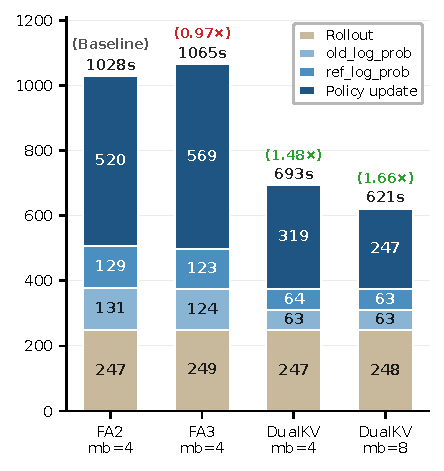
\includegraphics[width=\linewidth]{figures/longreason_step_breakdown_vertical.pdf}
\caption{Per-phase step breakdown.}
\label{fig:step-breakdown-main}
\vspace{-1em}
\end{wrapfigure}


\textbf{Setup.} We train Qwen3-8B on a single \texttt{p5.48xlarge} instance (8$\times$H100-SXM5-80GB) with FSDP2 in BF16 and gradient checkpointing. Rollout generation uses vLLM with tensor parallelism $=2$ and $N{=}32$ responses per prompt. Training uses \texttt{train\_batch\_size}${}=128$ and \texttt{ppo\_mini\_batch\_size}${}=64$ (both fixed across all configurations), and we sweep \texttt{ppo\_micro\_batch\_size\_per\_gpu} $\in \{4, 8\}$. Each configuration runs for 25 training steps with validation every 2 steps. Although the rollout factor is $N{=}32$, the token reduction ratio $\rho$ (Eq.~\ref{eq:rho}) is bounded by the \emph{micro-batch} size --- only sequences co-located in the same forward/backward pass share a prompt. With $P{=}8192$, $R{=}2048$: $\rho = 2.5\times$ at mb=4 and $\rho = 3.3\times$ at mb=8, setting upper bounds on the measured policy-update speedup.

\textbf{Comparisons.} We compare four configurations (\texttt{mb} = per-GPU micro-batch size): FA2 (mb=4), the largest micro-batch FA2 can handle (mb=8 OOMs); FA3 (mb=4), evaluating the Hopper-specific kernel; DualKV (mb=4), an apple-to-apple comparison; and DualKV (mb=8), a configuration FA2 cannot run.



\textbf{Results.} Table~\ref{tab:e2e-longreason} and Figure~\ref{fig:longreason-comparison} summarize both experiments. All configs track identical training accuracy curves (Figure~\ref{fig:longreason-comparison}A), confirming DualKV introduces no convergence degradation for either method (formal proof in Appendix~\ref{app:pipeline-invariance}).



\begin{figure}[!t]
\centering
\makebox[\textwidth][c]{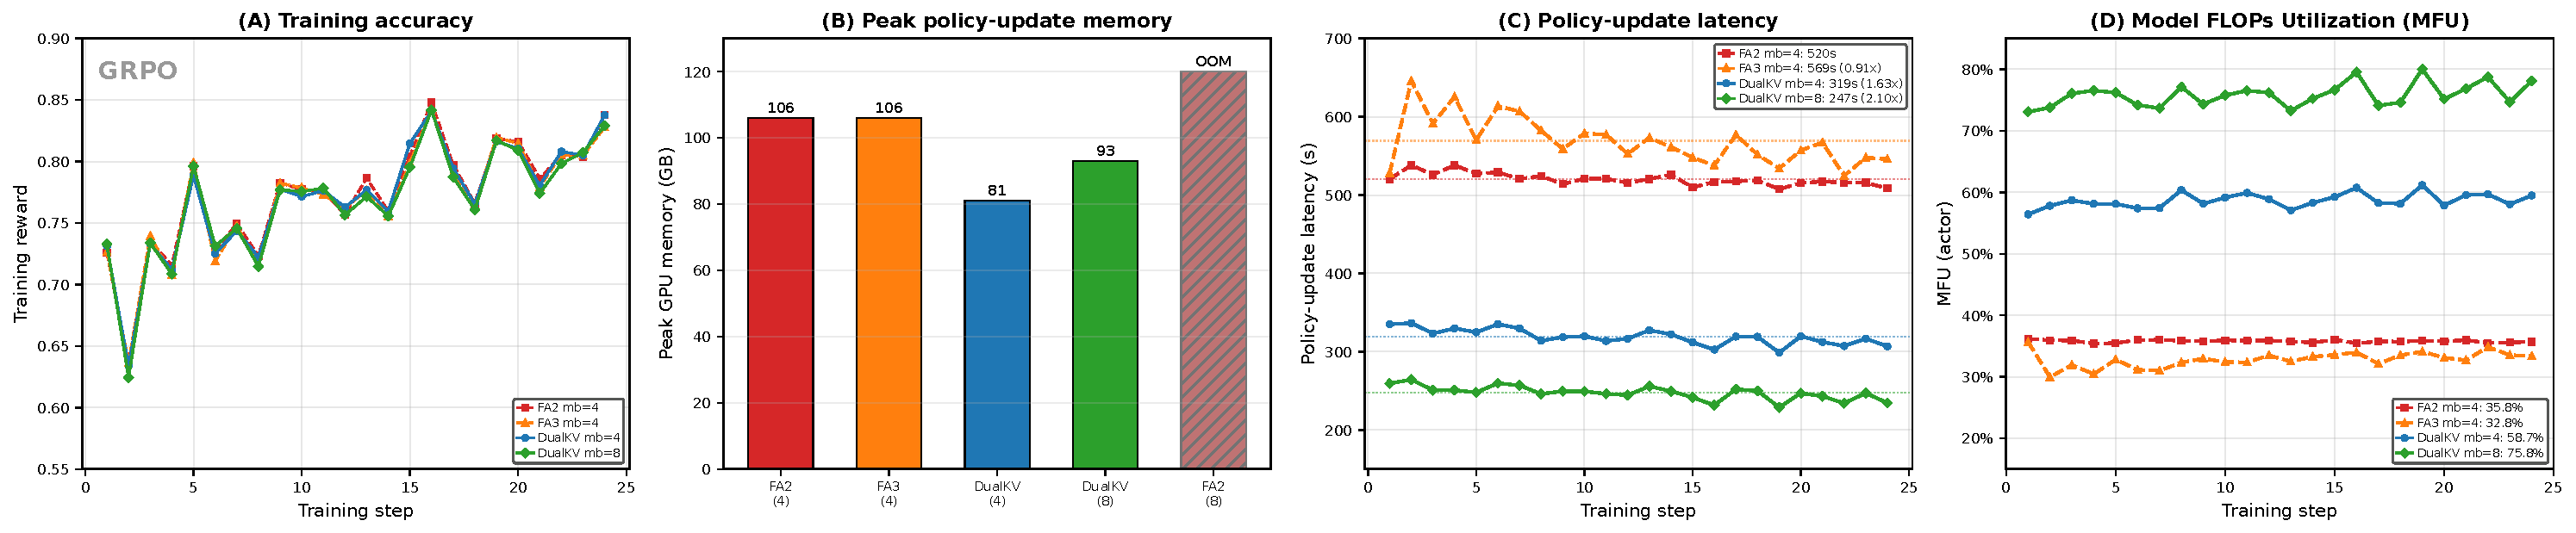
\includegraphics[width=1.0\textwidth]{figures/longreason_comparison_1x4.pdf}}
% \vspace{-0.5em}
\makebox[\textwidth][c]{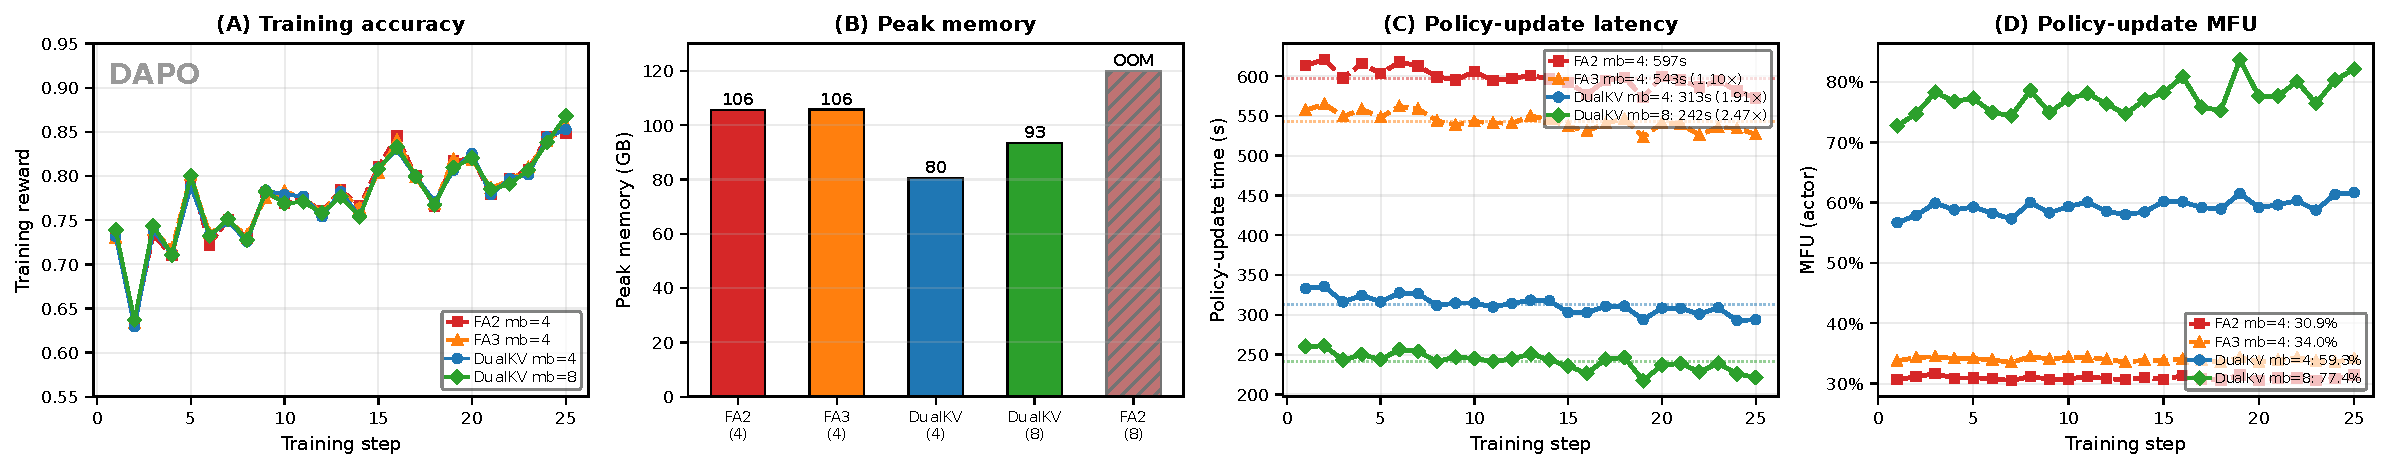
\includegraphics[width=1.0\textwidth]{figures/dapo_longreason_comparison_1x4.pdf}}
\caption{LongReason training (Qwen3-8B, 8$\times$H100), four configurations. \textbf{Top row}: GRPO ($N{=}32$, steps 1--24). \textbf{Bottom row}: DAPO ($N{=}32$, steps 1--25). Panels: \textbf{(A)}~Training reward --- all configs track identically. \textbf{(B)}~Peak memory. \textbf{(C)}~Policy-update latency. \textbf{(D)}~Policy-update MFU. GRPO: DualKV mb=8 achieves $2.09\times$ speedup, $75.8\%$ MFU. DAPO: $2.47\times$ speedup, $77.4\%$ MFU.}
\label{fig:longreason-comparison}
\end{figure}



% Legacy two-figure layout (replaced by fig:longreason-comparison).
\iffalse
\begin{figure}[ht]
\centering
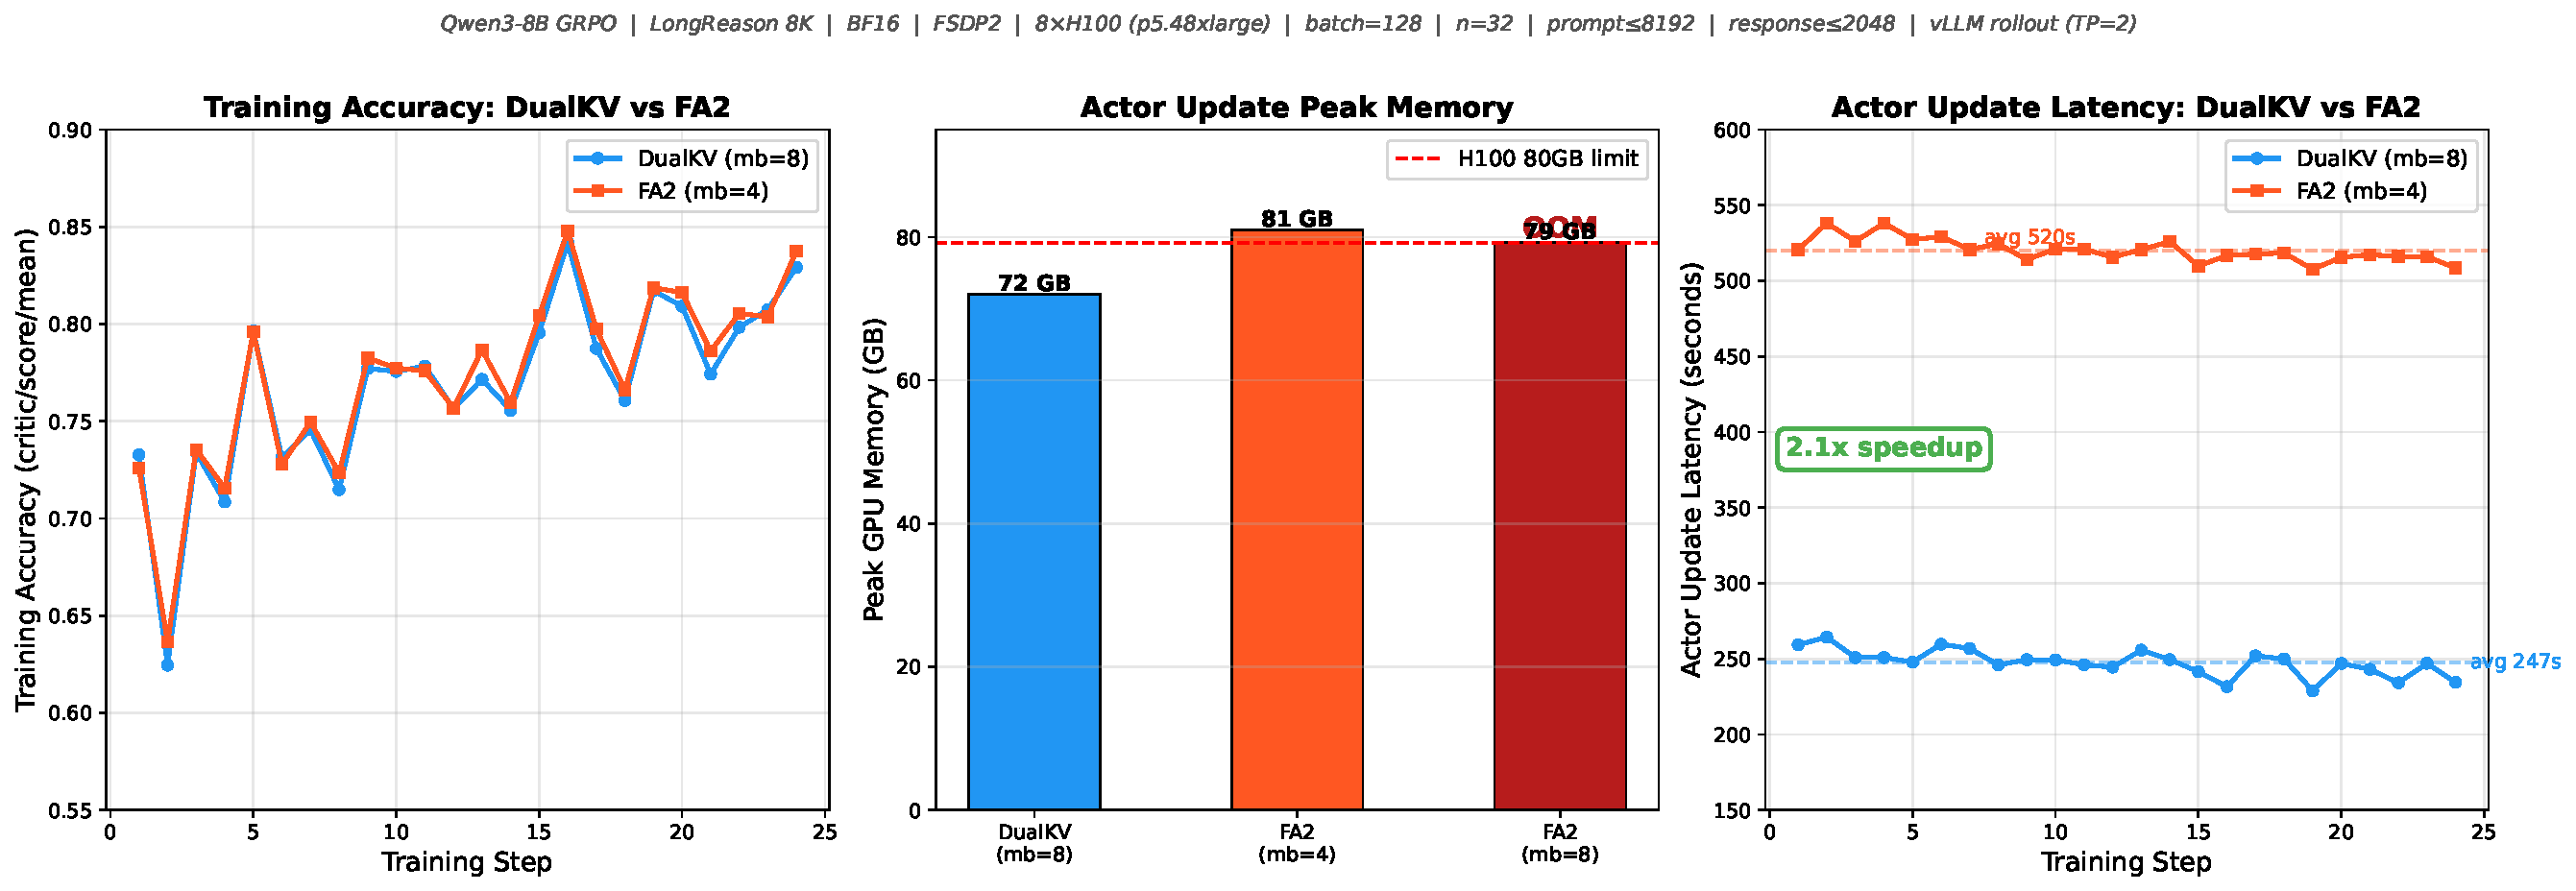
\includegraphics[width=\textwidth]{figures/dualkv_vs_fa2_comparison.pdf}
\caption{DualKV (mb=8) vs.\ FA2 (mb=4) on LongReason over 24 GRPO steps. \textbf{Left}: Training accuracy (critic score) --- both methods track identically. \textbf{Center}: Peak policy update memory --- FA2 at mb=8 exceeds the H100 80\,GB limit (OOM), while DualKV at mb=8 fits at 72\,GB. \textbf{Right}: Policy update latency per step --- DualKV averages 248\,s vs.\ FA2's 520\,s ($2.1\times$ speedup).}
\label{fig:longreason-mb8}
\end{figure}

\begin{figure}[ht]
\centering
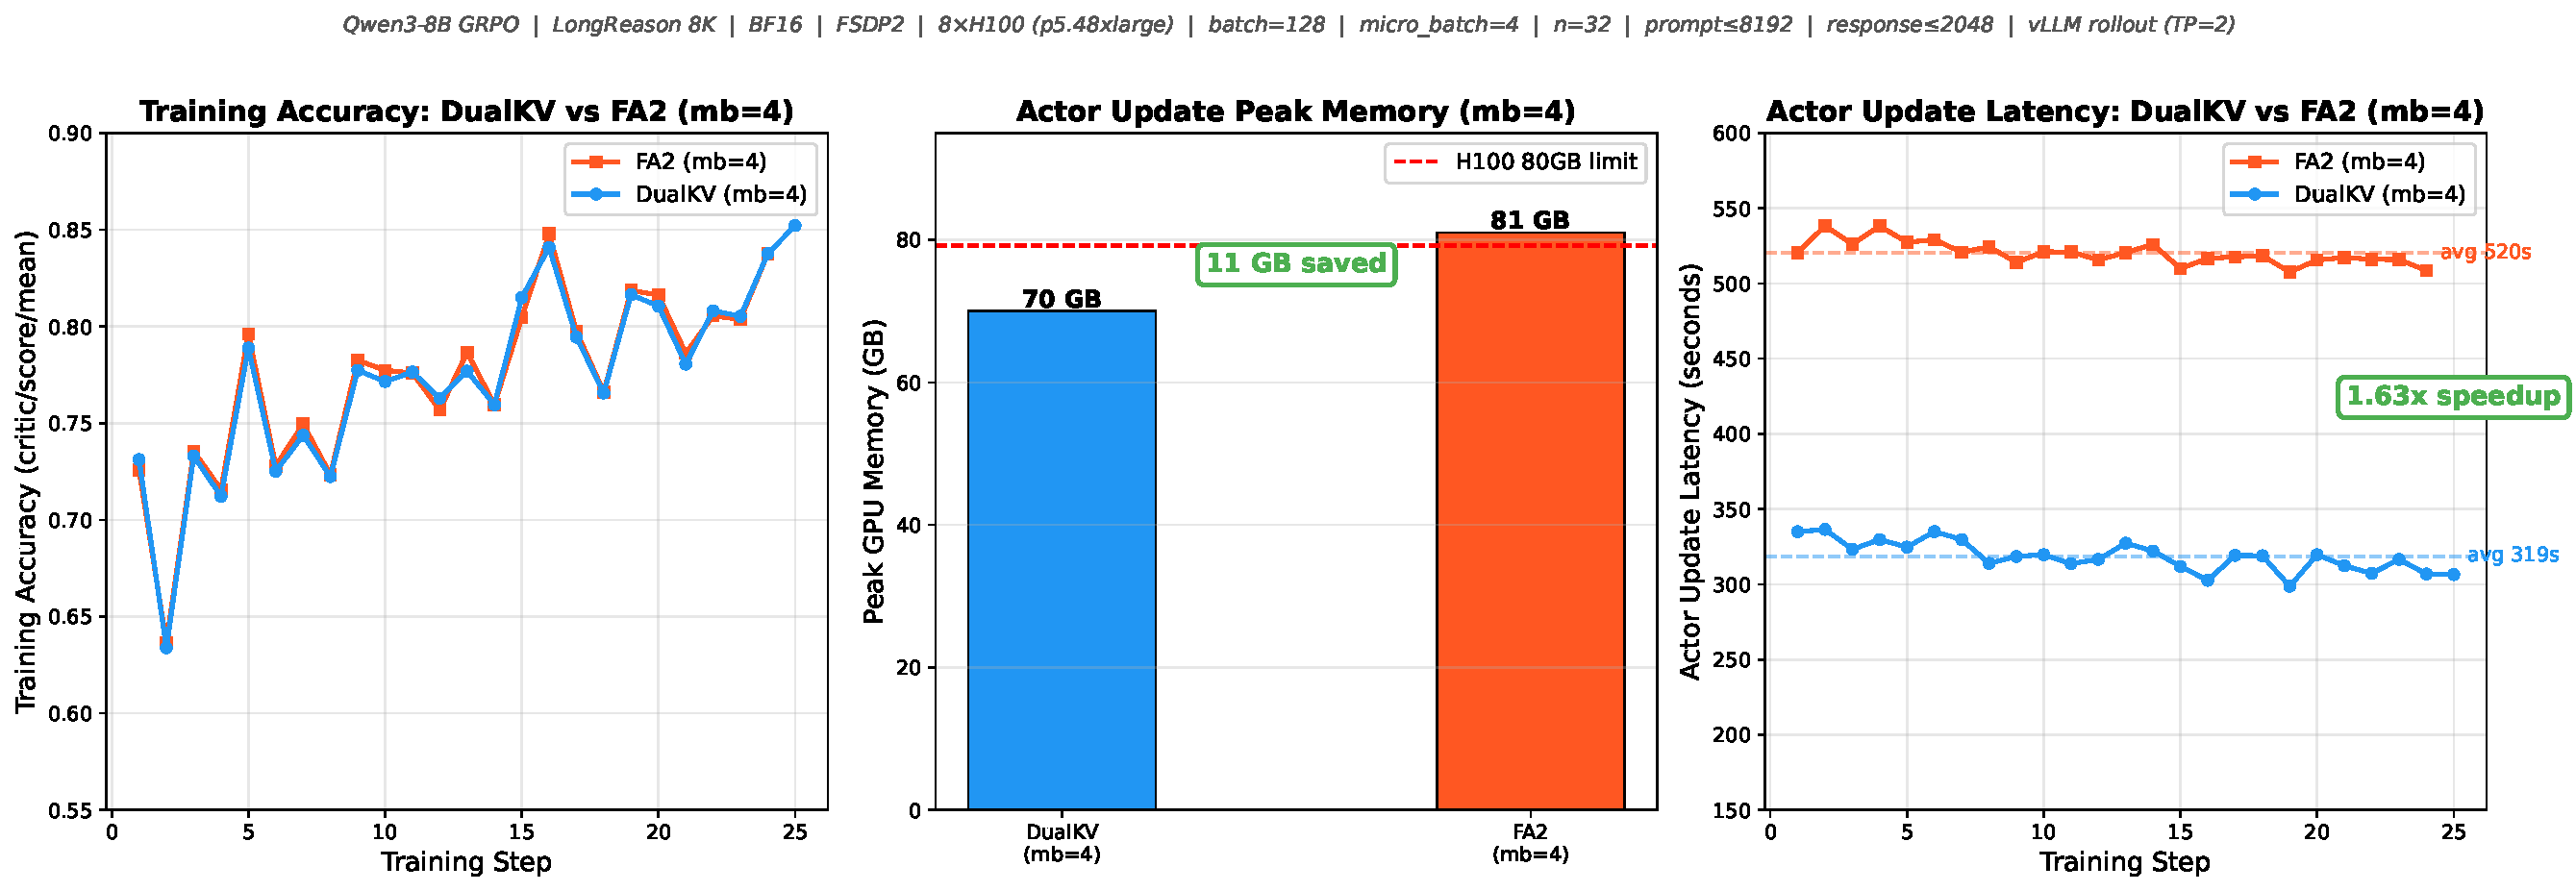
\includegraphics[width=\textwidth]{figures/dualkv_vs_fa2_mb4_comparison.pdf}
\caption{Apple-to-apple comparison: DualKV vs.\ FA2, both at mb=4, on LongReason over 25 GRPO steps. \textbf{Left}: Training accuracy tracks identically. \textbf{Center}: DualKV saves 11\,GB peak memory (70 vs.\ 81\,GB). \textbf{Right}: DualKV averages 319\,s vs.\ FA2's 520\,s ($1.63\times$ speedup), purely from KV deduplication without changing gradient accumulation.}
\label{fig:longreason-mb4}
\end{figure}
\fi

% \vspace{-0.5em}



\textbf{Speedups, memory, and MFU.} At mb=4, DualKV cuts policy-update time by $1.63\times$ (GRPO) and $1.91\times$ (DAPO), while reducing peak memory from $106$\,GB to $81$\,GB --- a 25\,GB reduction that brings the workload within the H100's 80\,GB physical HBM. FA2's 106\,GB allocation exceeds HBM capacity via memory oversubscription, degrading throughput. Doubling to mb=8 --- which FA2 OOMs on --- extends the speedup to $2.09\times$ (GRPO) and $2.47\times$ (DAPO), halving the gradient-accumulation passes per mini-batch ($2 \to 1$). Policy-update MFU rises from $36\%$/$31\%$ (FA2) to $76\%$/$77\%$ (DualKV mb=8) for GRPO/DAPO respectively --- a $2.1$--$2.5\times$ utilization gain. DAPO's higher speedups reflect the absence of the ref phase: the policy update dominates a larger fraction of step time, so DualKV's per-phase compression translates more directly to wall-clock gains.



\begin{wraptable}{r}{0.6\textwidth}
% \vspace{-1em}
\centering
\scriptsize
\setlength{\tabcolsep}{3pt}
\caption{End-to-end LongReason results. \texttt{Step} = total training-step time (s). \texttt{MFU} = policy-update Model FLOPs Utilization. Parentheses = speedup vs FA2 mb=4. Per-phase breakdown is in Figure~\ref{fig:step-breakdown-main}.}
\label{tab:e2e-longreason}
\begin{tabular}{@{}lc c c c c@{}}
\toprule
\textbf{Config} & \textbf{mb/GPU} & \textbf{Peak Mem} & \textbf{Step} & \textbf{MFU} & \textbf{Val Acc} \\
 & & \textbf{(GB)} & \textbf{(s)} & \textbf{(\%)} & \textbf{(step 24)} \\
\midrule
FA2      & 4 & 106\rlap{$^\dagger$} & 1017 (1.00$\times$) & 35.8 & 0.777 \\
FA3      & 4 & 106\rlap{$^\dagger$} & 1067 (0.95$\times$) & 32.8 & 0.793 \\
DualKV   & 4 & 81                  &  687 (1.48$\times$) & 58.8 & 0.780 \\
DualKV   & 8 & 93                  &  622 (1.64$\times$) & 75.8 & 0.780 \\
FA2      & 8 & \multicolumn{4}{c}{OOM during \texttt{loss.backward()}} \\
\bottomrule
\end{tabular}
\vspace{2pt}

{\scriptsize $^\dagger$PyTorch allocator reservation; actual HBM use stays within 80\,GB.}
\end{wraptable}
\textbf{End-to-end step speedup.} Total training step time drops $1.64\times$/$1.82\times$ (GRPO/DAPO) at mb=8. The remaining gap versus the per-phase speedups is explained by rollout generation (${\sim}240$\,s/step, unaffected by DualKV), whose share of step time grows as training phases accelerate --- DualKV shifts the bottleneck from the policy update to rollout generation (Figure~\ref{fig:step-breakdown-main}). Full per-phase DAPO breakdowns are in Appendix~\ref{app:dapo-longreason}.

\subsection{Multi-Node RL Training with MoE Models}
\label{sec:e2e-moe-multinode}

\begin{wrapfigure}{r}{0.5\textwidth}
\vspace{-1.5em}
\centering
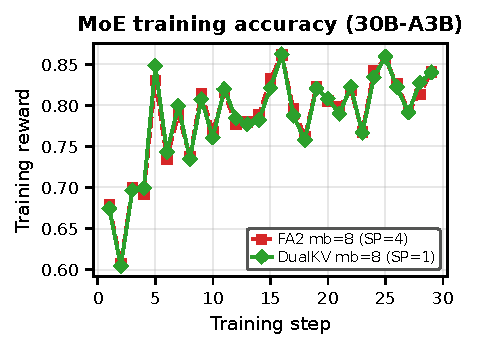
\includegraphics[width=\linewidth]{figures/moe_multinode_accuracy.pdf}
\caption{Per-step training accuracy.}
\label{fig:moe-accuracy}
\end{wrapfigure}
To validate DualKV at production scale with cross-node communication and MoE expert routing, we train Qwen3-30B-A3B~\citep{yang2025qwen3} with GRPO on two \texttt{p5.48xlarge} nodes (16$\times$H100 GPUs, Elastic Fabric Adapter): FSDP2 + BF16 + gradient checkpointing; rollout via vLLM (TP${=}2$, $N{=}32$). All runs: \texttt{train\_batch\_size}${=}128$, \texttt{ppo\_mini\_batch\_size}${=}64$, \texttt{ppo\_micro\_batch\_size\_per\_gpu}${=}8$, $P_{\max}{=}8192$, $R_{\max}{=}2048$. Timing is mean over 29 steps. We compare three configurations: DualKV (SP=1), no sequence parallelism; FA2 (SP=2), which OOMs during the first policy update; and FA2 (SP=4), the minimum SP that avoids OOM.

\textbf{Results.} Table~\ref{tab:e2e-moe-multinode} summarizes the three configurations. DualKV delivers a $3.82\times$ policy-update speedup and $3.38\times$ total step speedup over FA2 SP=4, without requiring sequence parallelism. Both configs track identical training accuracy curves (Figure~\ref{fig:moe-accuracy}), confirming DualKV introduces no convergence degradation at multi-node training scale (formal proof in Appendix~\ref{app:pipeline-invariance}).

\begin{table}[ht]
\centering
\scriptsize
\setlength{\tabcolsep}{4pt}
\caption{Wall-clock values are means over 29 steps; parenthesized values are speedups relative to FA2 SP=4.}
\label{tab:e2e-moe-multinode}
\begin{tabular}{@{}lc c c c c c c c c@{}}
\toprule
\textbf{Config} & \textbf{mb/GPU} & \textbf{SP} & \textbf{Peak Mem} & \textbf{Policy Update} & \textbf{old\_log\_prob} & \textbf{ref\_log\_prob} & \textbf{Rollout} & \textbf{Step} & \textbf{Val Acc} \\
 & & & \textbf{(GB)} & \textbf{(s)} & \textbf{(s)} & \textbf{(s)} & \textbf{(s)} & \textbf{(s)} & \textbf{(step 28)} \\
\midrule
DualKV  & 8 & 1 & 103\rlap{$^\dagger$} & 1078 (3.82$\times$) & 129 (3.45$\times$) & 142 (3.58$\times$) & 215 (1.00$\times$) & 1564 (3.38$\times$) & 0.774 \\
FA2     & 8 & 4 &  92\rlap{$^\dagger$} & 4115 (1.00$\times$) & 447 (1.00$\times$) & 507 (1.00$\times$) & 214 (1.00$\times$) & 5284 (1.00$\times$) & 0.802 \\
FA2     & 8 & 2 & \multicolumn{7}{c}{OOM during first \texttt{loss.backward()}} \\
\bottomrule
\end{tabular}
\vspace{2pt}

{\scriptsize $^\dagger$PyTorch allocator reservation; actual HBM use stays within 80\,GB.}
\end{table}

\textbf{Speedups at multi-node MoE scale.}
DualKV delivers a $3.82\times$ policy-update speedup and $3.38\times$ total-step speedup (5284\,s $\to$ 1564\,s, throughput 293 $\to$ 991 tokens/s). The larger gains versus the 8B single-node range ($1.63$--$2.09\times$) arise because (i) MoE expert GEMMs amplify the per-token savings from DualKV's $(N{-}1) \cdot P$ reduction, and (ii) DualKV eliminates the all-to-all communication that FA2 with SP=4 pays on every attention call. Over 29 steps, DualKV completes in 12.6 hours vs.\ 42.6 hours for FA2 SP=4 on the same 16-GPU cluster (${\sim}\$6$K saved at AWS \texttt{p5.48xlarge} on-demand list price). Figure~\ref{fig:moe-multinode-breakdown} (Appendix~\ref{app:additional-figures}) visualizes the phase-wise breakdown.

\textbf{Eliminating sequence parallelism.} DualKV's memory reduction enables training at SP=1, whereas FA2 OOMs at SP=2 and requires SP=4. This translates memory savings into additional speedup: DualKV avoids the per-call all-to-all communication that SP imposes, which is why end-to-end gains ($3.38\times$) exceed what token dedup alone would predict.

\subsection{Memory Scaling with Context Length}
\label{sec:memory-scaling}

To characterize how DualKV's advantage scales with prompt length, we sweep $P \in \{8\text{K}\text{--}96\text{K}\}$ and $\text{mb} \in \{4, 8, 16\}$ on Llama-3.1-8B (16$\times$H100). This experiment also validates that DualKV generalizes across model families (Llama here versus Qwen3 in Sections~\ref{sec:e2e-longreason}--\ref{sec:e2e-moe-multinode}).

\begin{wrapfigure}
{r}{0.55\textwidth}
\vspace{-1.5em}
\centering
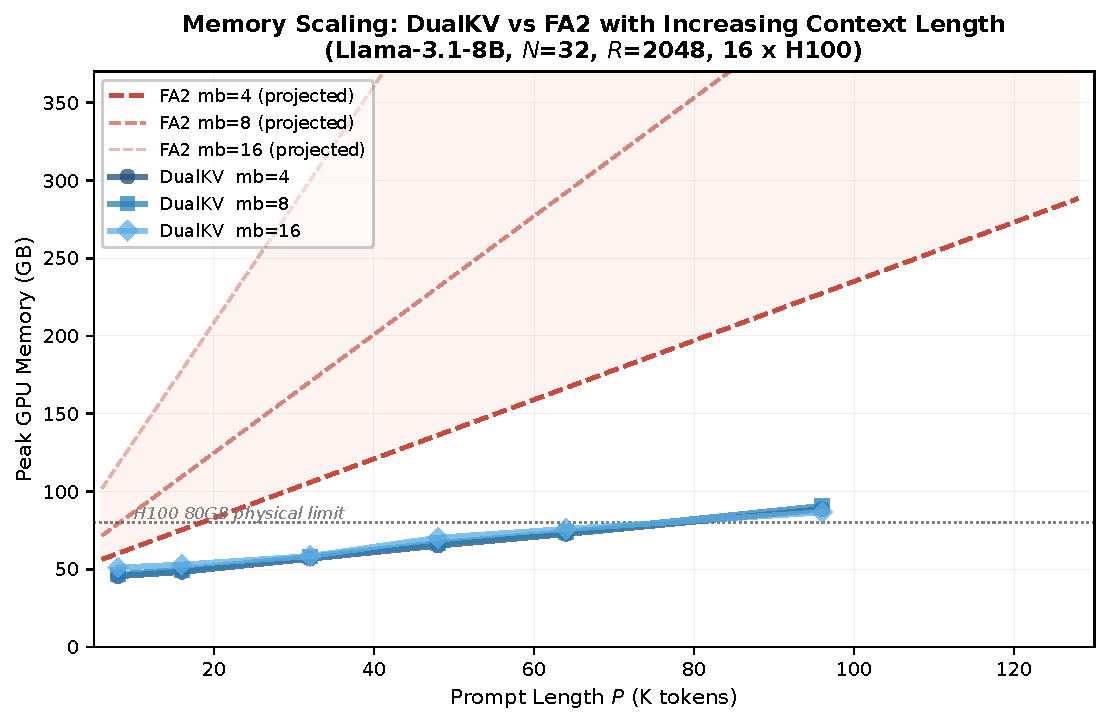
\includegraphics[width=\linewidth]{figures/memory_scaling_law.pdf}
\caption{Memory scaling: DualKV vs.\ FA2.}
\label{fig:memory-scaling-law-main}
\vspace{-1em}
\end{wrapfigure}
\textbf{Memory decouples from micro-batch size.} DualKV's memory follows $M_0 + c_P \cdot P + c_{\text{mb}R} \cdot \text{mb} \cdot R$: the prompt cost is paid once regardless of micro-batch size, so the three mb curves cluster tightly (Figure~\ref{fig:memory-scaling-law-main}). FA2's memory scales as $M_0 + c \cdot \text{mb} \cdot (P{+}R)$, diverging rapidly --- at $P{=}96\text{K}$, increasing mb from 4 to 16 adds only ${\sim}4$\,GB under DualKV ($<5\%$), whereas FA2 would require $225 \to 775$\,GB --- nearly $10\times$ the physical capacity of an H100. Practitioners can freely increase mb to maximize throughput without memory penalty in the long-prompt regime.



%----------------------------------------------------------------------
\section{Related Work}
%----------------------------------------------------------------------

\textbf{Efficient attention for long sequences.} FlashAttention~\citep{dao2022flashattention,dao2023flashattention2,shah2024flashattention3} reduces attention memory from $O(S^2)$ to $O(S)$ via tiling and online softmax; Ring attention~\citep{liu2023ringattention}, Ulysses~\citep{jacobs2023ulysses}, Megatron-SP~\citep{korthikanti2023reducing}, and Context Parallelism~\citep{dubey2024llama3} distribute sequences across GPUs via sequence parallelism. All are orthogonal to DualKV's within-GPU shared-prompt deduplication and compose with it.

\textbf{Shared-prompt optimization.} Paged attention~\citep{kwon2023vllm}, RadixAttention~\citep{zheng2023sglang}, and bifurcated attention~\citep{athiwaratkun2024bifurcated} share prompt KV for inference only. Prefix Grouper~\citep{liu2025prefixgrouper} is a framework-level data reorganization that applies the shared-prompt decomposition to RL policy updates but replicates $K, V$ $N$ times before the attention call, retaining $O(N \cdot P \cdot d)$ memory at the kernel level. DualKV contributes the kernel-level primitive that eliminates this replication: a FlashAttention variant that reads shared KV from a single physical buffer and accumulates gradients from $N$ concurrent sequences via fp32 atomic writes, fully realizing the decomposition's memory and compute savings for training (Appendix~\ref{app:prefix-grouper-comparison} shows DualKV is 2--4$\times$ faster and uses 3--5$\times$ less memory than Prefix Grouper).

\textbf{RL training systems.} veRL~\citep{sheng2024verl}, OpenRLHF~\citep{hu2024openrlhf}, and TRL~\citep{vonwerra2020trl} implement PPO~\citep{schulman2017ppo}/GRPO~\citep{shao2024deepseekmath}/REINFORCE++~\citep{hu2025reinforceplusplus}/DAPO~\citep{yu2025dapo} policy updates by packing $N$ sequences with replicated prompts, without exploiting shared-prompt structure. DualKV is a drop-in replacement for the attention layer in these systems, requiring only data pipeline changes to group same-prompt responses.

% %----------------------------------------------------------------------
% \section{Discussion}
% \label{sec:discussion}
% %----------------------------------------------------------------------


%----------------------------------------------------------------------
\section{Conclusion}
%----------------------------------------------------------------------


DualKV eliminates the redundant prompt replication in RL policy updates by introducing a two-region FlashAttention kernel that reads shared KV from a single physical buffer, paired with a data-pipeline redesign that extends the token reduction to the entire model with provable gradient equivalence. Across dense and MoE models, DualKV achieves $2$--$3.8\times$ policy-update speedup, raises MFU from $36\%$ to $76\%$, and eliminates the need for sequence parallelism at long contexts. DualKV shifts the RL training bottleneck from the policy update to rollout generation. The current design assumes a single shared prefix per micro-batch group and benefits scale with $P/R$. Generalizing the kernel to arbitrary tree structures with shared sub-graphs (e.g., multi-turn conversations with partially overlapping prefixes or tree-of-thought search) would lift the single-prefix constraint. Future directions also include composing DualKV with Ulysses SP for ultra-long contexts and porting to FA3/Hopper and FA4/Blackwell backends. Our implementation is open-sourced at \textcolor{blue}{\url{https://github.com/amazon-science/dualkv-flash-attn-for-rl}}.


\bibliographystyle{plainnat}
\bibliography{refs}

\appendix

%----------------------------------------------------------------------
\section{DualKV Formal Derivation}
\label{app:dualkv-math}
%----------------------------------------------------------------------

This appendix provides a self-contained mathematical derivation of the DualKV forward and backward passes and proves equivalence to the FA2 baseline.

\subsection{Setup and Notation}

Consider $N$ sequences sharing a prompt of $P$ tokens. Sequence $i$ has $R_i$ response tokens, with total length $S_i = P + R_i$. Let $T = P + \sum_{i=1}^N R_i$ denote the total packed token count.

In a standard transformer layer, let $h \in \mathbb{R}^{T \times D}$ denote the hidden states after the input norm. The QKV projection produces:
\begin{equation}
  Q = h W_Q, \quad K = h W_K, \quad V = h W_V
\end{equation}
where $W_Q \in \mathbb{R}^{D \times Hd}$, $W_K \in \mathbb{R}^{D \times H_k d}$, $W_V \in \mathbb{R}^{D \times H_k d}$, with $H$ query heads, $H_k$ KV heads, and head dimension $d$.

\subsection{Prompt Hidden State Invariant}
\label{app:prompt-invariant}

\begin{claim}[Prompt Hidden State Invariant]
In a decoder-only model, for any prompt position $j < P$, the hidden state $h_j$ is identical across all $N$ sequences at every layer.
\end{claim}

\begin{proof}
By induction on layers. At the embedding layer, prompt tokens are shared, so $h_j^{(i)} = h_j$ for all $i$. Suppose the invariant holds at the input to layer $\ell$. Every operation in the layer preserves it:
\begin{itemize}
  \item \textbf{RMSNorm}: per-token, so $\text{Norm}(h_j^{(i)}) = \text{Norm}(h_j)$ for all $i$.
  \item \textbf{QKV projection}: linear per-token, so $Q_j^{(i)} = Q_j$, $K_j^{(i)} = K_j$, $V_j^{(i)} = V_j$.
  \item \textbf{RoPE}: depends only on position index $j$, applied per-token.
  \item \textbf{Causal attention}: for $j < P$, the causal mask restricts attention to keys at positions $\{0, \ldots, j\}$, all prompt positions with identical $K$ and $V$. Combined with $Q_j^{(i)} = Q_j$ from the QKV-projection step, the attention output satisfies $O_j^{(i)} = O_j$ for all $i$.
  \item \textbf{Output projection, residual, MLP}: all per-token or element-wise.
\end{itemize}
The invariant holds at the output of layer $\ell$, completing the induction.
\end{proof}

\subsection{Forward Pass}

\paragraph{Packing.} We represent the micro-batch as a single packed sequence:
\begin{equation}
  \mathbf{x} = [\underbrace{p_0, \ldots, p_{P-1}}_{\text{prompt}},\; \underbrace{r_0^{(1)}, \ldots, r_{R_1-1}^{(1)}}_{\text{response 1}},\; \ldots,\; \underbrace{r_0^{(N)}, \ldots, r_{R_N-1}^{(N)}}_{\text{response } N}]
\end{equation}

All per-token operations process $T = P + \sum_i R_i$ tokens, saving $(N{-}1) \cdot P$ tokens versus the standard $\sum_i S_i = NP + \sum_i R_i$ layout.

\paragraph{QKV split.} After the QKV projection on $T$ tokens, we split at the prompt boundary $P$ (zero-copy tensor views):
\begin{align}
  Q_c &= Q_{[0:P]}, \quad K_c = K_{[0:P]}, \quad V_c = V_{[0:P]} \label{eq:ctx-split} \\
  Q_d &= Q_{[P:T]}, \quad K_d = K_{[P:T]}, \quad V_d = V_{[P:T]} \label{eq:dec-split}
\end{align}

\paragraph{Call 1: Context self-attention.} Standard causal attention over the $P$ prompt tokens, computed once:
\begin{equation}
  O_c = \text{CausalAttn}(Q_c, K_c, V_c) \in \mathbb{R}^{P \times H \times d}
  \label{eq:call1}
\end{equation}

\paragraph{Call 2: Decoded attention (DualKV kernel).} For sequence $i$ and decoded position $r \in \{0, \ldots, R_i - 1\}$, the query attends to the full key-value sequence $[K_c;\, K_d^{(i)}]$ with causal masking at logical position $P + r$:
\begin{equation}
  O_d^{(i)}[r] = \sum_{j=0}^{P + r} \alpha_j^{(i,r)} \cdot v_j
  \label{eq:call2}
\end{equation}
where $v_j$ indexes into $[V_c;\, V_d^{(i)}]$ and the attention weights are:
\begin{equation}
  \alpha_j^{(i,r)} = \frac{\exp\!\big(q_r^{(i)} \cdot k_j / \sqrt{d}\big)}{\sum_{j'=0}^{P+r} \exp\!\big(q_r^{(i)} \cdot k_{j'} / \sqrt{d}\big)}
\end{equation}

The \texttt{context\_seqlen}${}= P$ parameter shifts the kernel's internal position counter so that decoded query at kernel index $r$ maps to logical position $P + r$, ensuring:
\begin{itemize}
  \item All $P$ context positions are unmasked ($j < P \leq P + r$).
  \item Decoded positions are causally masked ($j \leq P + r$).
\end{itemize}

\paragraph{Reassembly.} The final attention output is:
\begin{equation}
  O = [O_c;\, O_d] \in \mathbb{R}^{T \times H \times d}
\end{equation}
which flows through $W_O$, residual addition, and MLP on $T$ tokens.

\subsection{Backward Pass}

Let $\mathcal{L}$ denote the training loss (computed only over response tokens). We receive $\partial \mathcal{L}/\partial O \in \mathbb{R}^{T \times H \times d}$ and split it:
\begin{equation}
  \frac{\partial \mathcal{L}}{\partial O_c} = \left(\frac{\partial \mathcal{L}}{\partial O}\right)_{\![0:P]}, \quad
  \frac{\partial \mathcal{L}}{\partial O_d} = \left(\frac{\partial \mathcal{L}}{\partial O}\right)_{\![P:T]}
\end{equation}

Note that $\partial \mathcal{L}/\partial O_c \neq 0$ in general: even though the loss is on response tokens only, gradients propagate back to prompt positions through subsequent layers' residual connections.

\paragraph{Call 2 backward (DualKV kernel).} Given $\partial \mathcal{L}/\partial O_d$ and the saved tensors from the forward pass, the backward produces:
\begin{align}
  \frac{\partial \mathcal{L}}{\partial Q_d},\quad
  \frac{\partial \mathcal{L}}{\partial K_d},\quad
  \frac{\partial \mathcal{L}}{\partial V_d}
\end{align}
and gradients with respect to the shared context KV:
\begin{align}
  \left(\frac{\partial \mathcal{L}}{\partial K_c}\right)_{\!d} &= \sum_{i=1}^{N} \sum_{r=0}^{R_i - 1} \sum_{h} \frac{\partial \mathcal{L}}{\partial O_d^{(i)}[r,h]} \cdot \frac{\partial O_d^{(i)}[r,h]}{\partial K_c} \label{eq:dkc-dec} \\
  \left(\frac{\partial \mathcal{L}}{\partial V_c}\right)_{\!d} &= \sum_{i=1}^{N} \sum_{r=0}^{R_i - 1} \sum_{h} \frac{\partial \mathcal{L}}{\partial O_d^{(i)}[r,h]} \cdot \frac{\partial O_d^{(i)}[r,h]}{\partial V_c} \label{eq:dvc-dec}
\end{align}

\paragraph{Implementation: fp32 gradient accumulation.}
The summation over $N$ sequences in Eq.~\ref{eq:dkc-dec}--\ref{eq:dvc-dec} introduces a concurrent-write pattern absent from standard FlashAttention: the single shared $dK_c$ and $dV_c$ buffer has no batch offset, yet $N$ thread blocks (one per decoded sequence) concurrently compute partial contributions to the same context positions. DualKV resolves this with fp32 atomic accumulation in a dedicated accumulator buffer, followed by a cast kernel that converts the accumulator to bf16. The kernel-level description and pseudocode are given in Section~\ref{sec:kernel-backward} (Algorithms~\ref{alg:dualkv-backward}--\ref{alg:dualkv-bwd-convert}). For the purposes of the mathematical derivation that follows, the relevant property is that the kernel produces $(\partial\mathcal{L}/\partial K_c)_d = \sum_i \sum_r \sum_h \partial\mathcal{L}/\partial O_d^{(i)}[r,h] \cdot \partial O_d^{(i)}[r,h]/\partial K_c$ exactly (up to fp32 rounding) as stated in Eq.~\ref{eq:dkc-dec}--\ref{eq:dvc-dec}.

\paragraph{Call 1 backward (standard FA2).} Given $\partial \mathcal{L}/\partial O_c$, produces:
\begin{align}
  \frac{\partial \mathcal{L}}{\partial Q_c},\quad
  \left(\frac{\partial \mathcal{L}}{\partial K_c}\right)_{\!c},\quad
  \left(\frac{\partial \mathcal{L}}{\partial V_c}\right)_{\!c}
\end{align}

\paragraph{Gradient accumulation.} Since $K_c$ and $V_c$ are the \emph{same tensor objects} passed to both Call~1 and Call~2, PyTorch autograd accumulates their gradients:
\begin{align}
  \frac{\partial \mathcal{L}}{\partial K_c} &= \left(\frac{\partial \mathcal{L}}{\partial K_c}\right)_{\!c} + \left(\frac{\partial \mathcal{L}}{\partial K_c}\right)_{\!d} \label{eq:dkc-total} \\
  \frac{\partial \mathcal{L}}{\partial V_c} &= \left(\frac{\partial \mathcal{L}}{\partial V_c}\right)_{\!c} + \left(\frac{\partial \mathcal{L}}{\partial V_c}\right)_{\!d} \label{eq:dvc-total}
\end{align}

The full QKV gradients are then reassembled:
\begin{equation}
  \frac{\partial \mathcal{L}}{\partial Q} = \left[\frac{\partial \mathcal{L}}{\partial Q_c};\, \frac{\partial \mathcal{L}}{\partial Q_d}\right], \quad
  \frac{\partial \mathcal{L}}{\partial K} = \left[\frac{\partial \mathcal{L}}{\partial K_c};\, \frac{\partial \mathcal{L}}{\partial K_d}\right], \quad
  \frac{\partial \mathcal{L}}{\partial V} = \left[\frac{\partial \mathcal{L}}{\partial V_c};\, \frac{\partial \mathcal{L}}{\partial V_d}\right]
\end{equation}

These propagate through the QKV projection backward to produce $\partial \mathcal{L}/\partial h$ and $\partial \mathcal{L}/\partial W_Q$, $\partial \mathcal{L}/\partial W_K$, $\partial \mathcal{L}/\partial W_V$.

\subsection{Equivalence to the FA2 Baseline}
\label{sec:equiv-theorem}

\begin{theorem}[Gradient Equivalence]
The parameter gradients produced by DualKV are identical to those produced by the FA2 baseline.
\end{theorem}

\begin{proof}
In the standard approach, each sequence $i \in \{1, \ldots, N\}$ has its own copy of the prompt KV: $K_c^{(i)}, V_c^{(i)}$. The gradient of $K_c^{(i)}$ has two components:
\begin{equation}
  \frac{\partial \mathcal{L}}{\partial K_c^{(i)}} = \underbrace{g_{\text{self}}^{(i)}}_{\text{prompt self-attn}} + \underbrace{g_{\text{cross}}^{(i)}}_{\text{decoded} \to \text{context}}
\end{equation}

The parameter gradient from the $W_K$ projection at prompt positions is:
\begin{equation}
  \frac{\partial \mathcal{L}}{\partial W_K}\bigg|_{\text{prompt}} = \sum_{i=1}^{N} \left(\frac{\partial \mathcal{L}}{\partial K_c^{(i)}}\right)^\top h_c = \left(\sum_{i=1}^{N} \frac{\partial \mathcal{L}}{\partial K_c^{(i)}}\right)^\top h_c
  \label{eq:dwk-standard}
\end{equation}
where $h_c$ is the prompt hidden state (identical across $i$ by the invariant, so it factors out of the sum).

In DualKV, the single $K_c$ receives gradient (Eq.~\ref{eq:dkc-total}):
\begin{equation}
  \frac{\partial \mathcal{L}}{\partial K_c} = \left(\frac{\partial \mathcal{L}}{\partial K_c}\right)_{\!c} + \sum_{i=1}^{N} g_{\text{cross}}^{(i)}
\end{equation}

The parameter gradient is:
\begin{equation}
  \frac{\partial \mathcal{L}}{\partial W_K}\bigg|_{\text{prompt}}^{\text{DualKV}} = \left(\frac{\partial \mathcal{L}}{\partial K_c}\right)^\top h_c
  \label{eq:dwk-dualkv}
\end{equation}

It remains to show that Eq.~\ref{eq:dwk-standard} equals Eq.~\ref{eq:dwk-dualkv}, i.e.:
\begin{equation}
  \sum_{i=1}^{N} \left(g_{\text{self}}^{(i)} + g_{\text{cross}}^{(i)}\right) = \left(\frac{\partial \mathcal{L}}{\partial K_c}\right)_{\!c} + \sum_{i=1}^{N} g_{\text{cross}}^{(i)}
  \label{eq:to-show}
\end{equation}

This reduces to showing:
\begin{equation}
  \sum_{i=1}^{N} g_{\text{self}}^{(i)} = \left(\frac{\partial \mathcal{L}}{\partial K_c}\right)_{\!c}
  \label{eq:self-equiv}
\end{equation}

In the standard approach, $g_{\text{self}}^{(i)}$ is the gradient of $K_c^{(i)}$ from the context self-attention of sequence $i$. This depends on $\partial \mathcal{L}/\partial O_c^{(i)}$, which propagates back from subsequent layers. While the forward values at prompt positions are identical across $i$, the backward gradients $\partial \mathcal{L}/\partial O_c^{(i)}$ generally differ (each sequence $i$ has different response tokens producing different loss contributions).

In DualKV, the single prompt copy receives the \emph{aggregated} upstream gradient:
\begin{equation}
  \frac{\partial \mathcal{L}}{\partial O_c} = \sum_{i=1}^{N} \frac{\partial \mathcal{L}}{\partial O_c^{(i)}}
\end{equation}

This aggregation happens naturally through the residual stream: in the packed layout, prompt hidden states at layer $\ell{+}1$ receive gradients from all $N$ response branches propagating backward through subsequent layers. Since all intervening operations (norms, projections, MLP, residual) are per-token and \emph{linear in the backward pass}, the gradient at the prompt positions is exactly the sum over all $N$ sequences' contributions.

The context self-attention backward is linear in $\partial \mathcal{L}/\partial O_c$:
\begin{equation}
  \left(\frac{\partial \mathcal{L}}{\partial K_c}\right)_{\!c} = f_{\text{attn-bwd}}\!\left(\frac{\partial \mathcal{L}}{\partial O_c}\right) = f_{\text{attn-bwd}}\!\left(\sum_{i=1}^{N} \frac{\partial \mathcal{L}}{\partial O_c^{(i)}}\right) = \sum_{i=1}^{N} f_{\text{attn-bwd}}\!\left(\frac{\partial \mathcal{L}}{\partial O_c^{(i)}}\right) = \sum_{i=1}^{N} g_{\text{self}}^{(i)}
\end{equation}

where $f_{\text{attn-bwd}}$ denotes the attention backward function mapping $dO$ to $dK$, which is linear in $dO$ (since the forward values $Q_c, K_c, V_c$ are fixed during backward). This establishes Eq.~\ref{eq:self-equiv} and completes the proof.
\end{proof}

\subsection{Complexity Summary}

This subsection summarizes the per-component FLOPs and memory scaling of FA2 baseline vs.\ DualKV in asymptotic notation, abstracting the concrete numbers of Section~\ref{sec:training}. The table shows that the savings are dominated by the token-count reduction $T_{\text{std}} \to T_{\text{dk}}$: every per-token cost (norms, projections, MLP, KV storage, activation memory) shrinks by the ratio $\rho = T_{\text{std}}/T_{\text{dk}}$, and only attention has additional structural savings beyond that.

\begin{table}[ht]
\centering
\caption{Complexity comparison. $T_{\text{std}} = NP + \sum_i R_i$, $T_{\text{dk}} = P + \sum_i R_i$.}
\label{tab:complexity}
\begin{tabular}{@{}lll@{}}
\toprule
\textbf{Component} & \textbf{FA2 baseline} & \textbf{DualKV} \\
\midrule
Norms, projections, MLP & $O(T_{\text{std}} \cdot D^2)$ & $O(T_{\text{dk}} \cdot D^2)$ \\
Attention FLOPs & $\sum_i O(S_i^2 \cdot H \cdot d)$ & $O(P^2 Hd) + \sum_i O(R_i S_i Hd)$ \\
KV memory per layer & $O(T_{\text{std}} \cdot H_k \cdot d)$ & $O(T_{\text{dk}} \cdot H_k \cdot d)$ \\
Activation memory & $O(T_{\text{std}} \cdot D)$ & $O(T_{\text{dk}} \cdot D)$ \\
\bottomrule
\end{tabular}
\end{table}

When $P \gg R$ and $R_i = R$ for all $i$:
\begin{equation}
  \frac{T_{\text{std}}}{T_{\text{dk}}} = \frac{NP + NR}{P + NR} \xrightarrow{P \gg R} N
\end{equation}

The savings approach a factor of $N$ (the batch size) across all components --- norms, projections, MLP, attention, and activation memory --- yielding near-linear scaling.

% Appendix B (Framework-Level Memory Analysis) temporarily commented out —
% pending revision / empirical calibration from benchmark profile traces.
\iffalse
%----------------------------------------------------------------------
\section{Framework-Level Memory Analysis}
\label{app:framework-memory}
%----------------------------------------------------------------------

Appendix~\ref{app:dualkv-math} establishes the per-operation FLOPs savings. This appendix quantifies the \emph{memory} footprint, separating kernel-local savings (already reported in Table~\ref{tab:kernel-mem}) from framework-level savings that arise because the entire transformer layer --- norms, projections, MLP, residual stream --- now processes $T_{\text{dk}} = P + N_\mu R$ tokens instead of $T_{\text{std}} = N_\mu(P+R)$. Together they account for the 25\,GB peak-memory reduction observed in the LongReason apple-to-apple comparison (Section~\ref{sec:e2e-longreason}, mb=4).

\subsection{Setup}

We analyze a single transformer layer of Qwen3-8B at the LongReason mb=4 configuration: hidden size $D{=}4096$, query heads $H{=}32$, KV heads $H_k{=}8$, head dim $d{=}128$, FFN inner dim $d_{\text{ff}}{=}12288$, $N_\mu{=}4$ sequences per micro-batch, $P{=}8192$, $R{=}2048$, bf16 activations (2\,bytes/element). The per-micro-batch token counts are $T_{\text{std}} = 4 \cdot 10240 = 40960$ and $T_{\text{dk}} = 8192 + 4 \cdot 2048 = 16384$, giving $\rho = 2.5\times$ and token delta $\Delta T = T_{\text{std}} - T_{\text{dk}} = 24576$.

\subsection{Per-Layer Activation Footprint}

Following the selective-activation-recompute taxonomy of~\citet{korthikanti2023reducing}, each transformer layer saves the following bf16 activations during forward to be consumed by backward:

\begin{table}[ht]
\centering
\small
\caption{Per-layer activation memory saved by DualKV relative to $N_\mu$-copy FA2. Configuration as in Appendix~\ref{app:framework-memory}. $\Delta T = 24576$ tokens.}
\label{tab:framework-mem}
\begin{tabular}{@{}lllr@{}}
\toprule
\textbf{Activation} & \textbf{Shape/token} & \textbf{Bytes saved (per layer)} & \textbf{MB} \\
\midrule
Pre-attention RMSNorm input     & $D$                    & $2 D \cdot \Delta T$              & 192 \\
Q, K, V projections (pre-RoPE)  & $(H + 2 H_k) d$        & $2 (H + 2 H_k) d \cdot \Delta T$ & 288 \\
Attention output (pre-$W_O$)    & $H d$                  & $2 H d \cdot \Delta T$            & 192 \\
Residual 1 (post-attn add)      & $D$                    & $2 D \cdot \Delta T$              & 192 \\
Pre-MLP RMSNorm input           & $D$                    & $2 D \cdot \Delta T$              & 192 \\
MLP gate+up projections         & $2 d_{\text{ff}}$      & $4 d_{\text{ff}} \cdot \Delta T$  & 1152 \\
SwiGLU intermediate             & $d_{\text{ff}}$        & $2 d_{\text{ff}} \cdot \Delta T$  & 576 \\
MLP down projection output      & $D$                    & $2 D \cdot \Delta T$              & 192 \\
Residual 2 (post-MLP add)       & $D$                    & $2 D \cdot \Delta T$              & 192 \\
\midrule
\textbf{Total per layer}        &                        &                                     & \textbf{3168\,MB} \\
\textbf{Across 36 layers}       &                        &                                     & \textbf{114\,GB} \\
\bottomrule
\end{tabular}
\end{table}

This table counts an \emph{upper bound}: it assumes every listed tensor is retained for backward with no recomputation. In practice, gradient checkpointing drops a subset of activations in exchange for selective recomputation.

\subsection{Reconciliation with Measured Memory Reduction}

The LongReason experiment uses block-level gradient checkpointing: each transformer block retains only its input tensor at forward time, and re-runs the forward on backward to regenerate the intermediate activations. Under this policy the realized savings decompose as:

\begin{enumerate}
  \item \textbf{Retained block-input activations} across 36 blocks: $2 D \cdot \Delta T \cdot 36 = 6.9$\,GB. These are not recomputed and scale linearly with $\Delta T$.
  \item \textbf{Within-block scratch activations} at the one block currently in backward: bounded by a single row of Table~\ref{tab:framework-mem}'s within-block contributions ($3168 - 192 - 192 = 2784$\,MB of within-block scratch, of which the backward pass needs roughly a third simultaneously due to ordering), producing ${\sim}0.9$\,GB of transient savings.
  \item \textbf{Kernel-level attention-input savings} (Table~\ref{tab:kernel-mem}, rescaled to mb=4): eliminating the 3 redundant prompt-KV copies, prompt-Q copies, and prompt \texttt{softmax\_lse} across 36 layers transiently; peak contribution is small (${\sim}0.2$\,GB) because these tensors are freed between layers under gradient checkpointing.
  \item \textbf{Autograd graph and tensor metadata}: residual overhead from allocator fragmentation and the smaller number of saved tensors in the computation graph.
\end{enumerate}

Summing the first two components ($6.9 + 0.9 \approx 7.8$\,GB) accounts for a significant portion of the measured $25$\,GB reduction (Table~\ref{tab:e2e-longreason}); the remainder is attributable to the transient kernel-level savings (the large attention output tensors that FA2 materializes but DualKV avoids) and allocator-level effects. The dominant savings at the whole-training-step level come from the framework-wide token reduction (rows 1--9 of Table~\ref{tab:framework-mem}), not from the attention kernel alone.

\subsection{Why Kernel-Only Accounting Understates Savings}

A common misconception is that shared-prompt attention only saves attention-input memory. Table~\ref{tab:framework-mem} shows that MLP activations dominate: the four MLP-related rows contribute $1152 + 576 + 192 = 1920$\,MB per layer, roughly $2.9\times$ the attention-related activations ($192 + 288 + 192 = 672$\,MB). Because DualKV packs $T_{\text{dk}}$ tokens instead of $T_{\text{std}}$ through every operation --- not just attention --- \emph{all} of these activations shrink proportionally. The token-reduction ratio $\rho$ from Section~\ref{sec:training} therefore governs the full memory footprint, not merely the attention sub-computation, which is why end-to-end training benefits persist even when attention is a minority of the wall-clock budget.

\subsection{Scaling with Micro-Batch Size}

For fixed $P$ and $R$, the per-layer activation saving relative to the $N_\mu$-copy baseline is
\begin{equation}
  \Delta_{\text{mem}}(N_\mu) \;=\; c_{\text{layer}} \cdot (N_\mu - 1) \cdot P,
\end{equation}
where $c_{\text{layer}} \approx 132$\,kB/token is the per-token activation footprint (in bf16) summed across Table~\ref{tab:framework-mem}. The saving is linear in $N_\mu - 1$ at fixed $P$: doubling $N_\mu$ from 4 to 8 doubles the absolute memory saved, which is why mb=8 fits on an 80\,GB H100 under DualKV while mb=8 under standard packing triggers CUDA OOM (Table~\ref{tab:e2e-longreason}).
\fi
% End of commented-out Appendix B.

%----------------------------------------------------------------------
\section{Training-Step Gradient Equivalence}
\label{app:pipeline-invariance}
%----------------------------------------------------------------------

Appendix~\ref{app:dualkv-math} proves the DualKV kernel produces attention gradients identical to the FA2 baseline in exact arithmetic for any fixed packed input. This appendix lifts that kernel-level invariance to the training-step level. DualKV introduces two modifications to veRL's policy-update data pipeline, both motivated by the kernel's same-prompt-per-micro-batch packing contract:
\begin{enumerate}
  \item \textbf{Skip \texttt{balance\_batch}.} veRL's default pipeline reorders the rollout list by per-sample sequence length to equalize per-GPU token counts before dispatch. DualKV skips this step, since the seqlen permutation scatters rollouts from the same prompt across different GPUs, breaking the single-prompt packing the kernel requires. The global rollout multiset is unchanged; only its ordering and per-GPU partition differ.
  \item \textbf{Force \texttt{shuffle=False}} within the per-rank mini-batch iterator. Under the default pipeline, samples within each rank are reshuffled between PPO epochs. DualKV disables this to preserve contiguous prompt-grouped ordering across epochs.
\end{enumerate}

For one training step, let $B$ be the global multiset of $(p,r,A)$ triples produced by that step's rollout, where $p$ is a prompt, $r$ a sampled response, and $A=A(p,r)$ a scalar advantage. The policy-gradient estimator is $\hat g(B,\theta) = \sum_{(p,r,A) \in B} f(p,r,A,\theta)$, covering standard RL objectives (PPO, GRPO, DAPO). Let $\mathcal{P}_{\text{def}}$ denote veRL's default pipeline and $\mathcal{P}_{\text{dk}}$ the DualKV pipeline.

\begin{theorem}[No systematic bias at training-step aggregate]
For any parameters $\theta$,
\begin{equation}
  \sum_{(p,r,A) \in B} f^{\mathcal{P}_{\text{def}}}(p,r,A,\theta) \;=\; \sum_{(p,r,A) \in B} f^{\mathcal{P}_{\text{dk}}}(p,r,A,\theta) \qquad \text{in exact arithmetic.}
\end{equation}
\end{theorem}

\begin{proof}
The per-sample gradient $f(p,r,A,\theta)$ depends on $\theta$, the advantage $A$, and the per-token log-probabilities $\pi_\theta(r \mid p)$. Advantages are computed upstream of the policy update and are pipeline-independent. The kernel-level equivalence theorem of Appendix~\ref{app:dualkv-math} establishes the primary lemma we rely on: log-probabilities and their gradients at response positions are identical under $\mathcal{P}_{\text{def}}$ and $\mathcal{P}_{\text{dk}}$ for any fixed sample. Hence $f^{\mathcal{P}_{\text{def}}}(p,r,A,\theta) = f^{\mathcal{P}_{\text{dk}}}(p,r,A,\theta)$ termwise. The two pipeline modifications are both permutations of the rollout list, so the global multiset $B$ is the same under both pipelines. The equation follows by termwise equality and order-invariance of finite sums.
\end{proof}

%----------------------------------------------------------------------
\section{Theoretical Speedup and Memory Analysis}
\label{app:theoretical-analysis}
%----------------------------------------------------------------------

This appendix derives per-layer kernel-level memory savings and the closed-form attention speedup ratio for DualKV. These are theoretical ceilings; measured end-to-end numbers are in Sections~\ref{sec:e2e-longreason}--\ref{sec:e2e-moe-multinode} (and Appendix~\ref{app:gsm8k-shortprompt}).

\subsection{Memory Savings}
\label{app:theoretical-memory}

Per layer, the DualKV kernel avoids storing $N{-}1$ redundant copies of three tensors that an equivalent $N$-copy FA2 call would materialize:

\begin{table}[ht]
\centering
\small
\caption{Kernel-level memory savings per layer relative to an $N$-copy FA2 call over the same packed batch. Configuration: Qwen3-8B ($N{=}8$, $P{=}16384$, $R{=}2048$, $H{=}32$, $H_k{=}8$, $d{=}128$) in bf16.}
\label{tab:kernel-mem}
\begin{tabular}{@{}lll@{}}
\toprule
\textbf{Tensor saved} & \textbf{Per-layer savings (bytes)} & \textbf{Numerical} \\
\midrule
$K_c, V_c$ (shared prompt KV)         & $2 \cdot (N{-}1) \cdot P \cdot H_k \cdot d \cdot 2$ & 469\,MB \\
$Q$ at prompt positions (avoided vs.\ FA2 baseline) & $(N{-}1) \cdot P \cdot H \cdot d \cdot 2$ & 940\,MB \\
\texttt{softmax\_lse} for prompt positions & $(N{-}1) \cdot P \cdot H \cdot 4$              & 14\,MB \\
\midrule
\textbf{Total per layer}              &                                                      & \textbf{1423\,MB} \\
\bottomrule
\end{tabular}
\end{table}

These are \emph{kernel-level} savings: they count the per-layer attention-input tensors ($Q$ at prompt positions, $K_c$, $V_c$) and the prompt-position \texttt{softmax\_lse} that an FA2 baseline would materialize $N$ times and DualKV materializes once. DualKV's single-prompt packing also reduces framework-level activation memory across every per-token operation (norms, QKV/output projections, MLP, residual stream), since these now process $P + NR$ tokens instead of $N(P+R)$.

\subsection{Speedup Scaling}
\label{app:theoretical-speedup}

The attention speedup ratio scales approximately as:
\begin{equation}
  \text{Speedup}_{\text{attn}} \approx \frac{N \cdot S^2}{P^2 + N \cdot R \cdot S} = \frac{N(P+R)^2}{P^2 + NR(P+R)}
\end{equation}

For $P \gg R$, this simplifies to $\approx N$, meaning DualKV approaches a linear speedup in batch size as prompt length dominates. For $P{=}32\text{K}$, $R{=}2\text{K}$, $N{=}16$: theoretical speedup is $6.1\times$, measured fwd+bwd is $5.48\times$ (90\% efficiency). The consistent speedup across forward and backward passes confirms that the theoretical FLOPs analysis (Section~\ref{sec:training}) applies equally to both directions.

The end-to-end training speedup is lower than this kernel-level ceiling, as attention is only one component of the training step (alongside generation, projections, MLP, optimizer, and communication). The token reduction ratio $\rho$ (Section~\ref{sec:training}) provides an upper bound on the full-model speedup.

\subsection{Token Reduction Ratio \texorpdfstring{$\rho$}{ρ}: Scaling Analysis and Regimes}
\label{app:rho-scaling}

The token reduction ratio of DualKV over standard attention is:
\begin{equation}
  \rho = \frac{T_{\text{std}}}{T_{\text{dk}}} = \frac{N(P + R)}{P + NR}
  \label{eq:rho}
\end{equation}

This ratio governs the speedup across \emph{all} model components (norms, projections, MLP, activation memory), not just attention. We analyze its behavior along the two key axes: rollout factor $N$ and prompt-to-response ratio $P/R$.

\paragraph{Scaling with $N$ (rollout factor).} Fixing $P$ and $R$, taking the limit:
\begin{equation}
  \lim_{N \to \infty} \rho = \lim_{N \to \infty} \frac{N(P+R)}{P + NR} = \frac{P + R}{R} = 1 + \frac{P}{R}
\end{equation}

For large $N$, the speedup saturates at $1 + P/R$. With $P{=}16\text{K}$, $R{=}2\text{K}$: ceiling is $9\times$. Increasing $N$ beyond this point yields diminishing returns --- the bottleneck shifts to decoded-token compute $O(NR)$ which scales linearly in both approaches.

\paragraph{Scaling with $P/R$ (prompt length ratio).} Fixing $N$ and $R$, as $P \to \infty$:
\begin{equation}
  \lim_{P \to \infty} \rho = \lim_{P \to \infty} \frac{NP + NR}{P + NR} = N
\end{equation}

For long prompts, the speedup approaches $N$ --- near-linear in the rollout factor. This is the regime where DualKV is most impactful: the $(N{-}1)P$ redundant prompt tokens dominate total compute.

\paragraph{Concrete scenarios.} Table~\ref{tab:scenarios} shows the token reduction ratio $\rho$ for representative RL training configurations.

\begin{table}[ht]
\centering
\small
\caption{Token reduction ratio $\rho = T_{\text{std}} / T_{\text{dk}}$ for various $(N, P, R)$ configurations.}
\label{tab:scenarios}
\begin{tabular}{@{}rrrrl@{}}
\toprule
$N$ & $P$ & $R$ & $\rho$ & \textbf{Regime} \\
\midrule
8  & 2K   & 2K  & 1.8$\times$ & Short prompt, moderate rollout \\
8  & 16K  & 2K  & 4.5$\times$ & Long prompt, moderate rollout \\
8  & 64K  & 512 & 7.6$\times$ & Very long prompt \\
16 & 16K  & 2K  & 6.0$\times$ & Long prompt, large rollout \\
32 & 4K   & 2K  & 2.8$\times$ & Short prompt, very large rollout \\
32 & 16K  & 2K  & 7.2$\times$ & Long prompt, very large rollout \\
16 & 32K  & 2K  & 8.5$\times$ & Very long prompt, large rollout \\
16 & 64K  & 512 & 14.3$\times$ & Ultra-long prompt, large rollout \\
\bottomrule
\end{tabular}
\end{table}

Two regimes emerge where DualKV provides substantial benefits:
\begin{enumerate}
  \item \textbf{Large rollout factor} ($N \geq 16$): Common in GRPO and DAPO, where generating many candidate responses per prompt improves reward signal quality. At $N{=}32$ with $P{=}16\text{K}$, the reduction reaches $7.2\times$.
  \item \textbf{Long prompts} ($P \geq 16\text{K}$): Prevalent in agentic tasks, repository-level code generation, and multi-turn dialogue. At $P{=}64\text{K}$, even moderate rollout ($N{=}8$) yields $7.6\times$ reduction, and $N{=}16$ reaches $14.3\times$.
\end{enumerate}

%----------------------------------------------------------------------
\section{Software Environment}
\label{app:software-stack}
%----------------------------------------------------------------------

All kernel-level benchmarks (Section~\ref{sec:kernel-speedup}) and end-to-end GRPO training runs (Sections~\ref{sec:e2e-longreason}--\ref{sec:e2e-moe-multinode} and Appendix~\ref{app:gsm8k-shortprompt}) use an identical Python virtual environment. Configuration flags (\texttt{use\_dualkv}, \texttt{ulysses\_sequence\_parallel\_size}, \texttt{attn\_implementation}) are the only variables that differ between runs.

\begin{table}[ht]
\centering
\small
\caption{Software stack used across all experiments. ``DualKV build'' indicates our fork of \texttt{flash\_attn} 2.8.4 with the DualKV kernel (Section~\ref{sec:kernel}) added; base FA2 behavior is unchanged. ``DualKV integration'' indicates our patch to \texttt{verl} 0.7.0 that adds the data-pipeline changes (Section~\ref{sec:dualkv-packing}) and actor/trainer hooks needed to use the DualKV kernel.}
\label{tab:software-stack}
\begin{tabular}{@{}ll@{}}
\toprule
\textbf{Package} & \textbf{Version} \\
\midrule
Python               & 3.12 \\
\texttt{torch}       & 2.9.0+cu128 \\
\texttt{vllm}        & 0.12.0 \\
\texttt{flash\_attn} & 2.8.4 (DualKV build) \\
\texttt{verl}        & 0.7.0 (DualKV integration) \\
\texttt{transformers}& 4.57.6 \\
\texttt{ray}         & 2.55.1 \\
NCCL                 & 2.27.5 \\
\bottomrule
\end{tabular}
\end{table}

The veRL patch (${\sim}1200$ lines across 10 files) modifies the actor's forward pass, the trainer's data pipeline (skipping \texttt{balance\_batch}, enforcing prompt-grouping), and a monkey-patch hook that installs the DualKV attention call on supported model classes. Both the \texttt{flash\_attn} and \texttt{verl} patches are available at \textcolor{blue}{\url{https://github.com/amazon-science/dualkv-flash-attn-for-rl}}.

%----------------------------------------------------------------------
\section{Additional Experiments}
\label{app:additional-training}
%----------------------------------------------------------------------

\subsection{GRPO Training on GSM8K (Short Prompts)}
\label{app:gsm8k-shortprompt}

This appendix presents our short-prompt validation experiment (referenced in Section~\ref{sec:experiments} introduction). The experiment stress-tests DualKV in the low-$\rho$ regime ($\rho = 1.8$--$3.8\times$), where kernel-level speedups are modest but memory savings still extend the feasible training frontier.

We evaluate DualKV in end-to-end GRPO training using the veRL framework on GSM8K~\citep{cobbe2021gsm8k}, comparing against standard FA2 packing across a range of prompt lengths.

\paragraph{Setup.} We train Qwen3-8B~\citep{yang2025qwen3} with GRPO on an 8-node cluster of NVIDIA A100-SXM4-40GB GPUs (64 GPUs total). The model is sharded via FSDP across 32 data-parallel ranks (tensor parallelism $=2$), with gradient checkpointing enabled and optimizer states offloaded to CPU. Each training step consists of: (1)~rollout generation via vLLM ($N{=}8$ responses per prompt, $R_{\max}{=}256$), (2)~log-probability computation, and (3)~policy update with gradient accumulation (micro-batch size $=8$ per GPU). We use \texttt{ppo\_mini\_batch\_size}${}=128$ and \texttt{train\_batch\_size}${}=512$.

\paragraph{Dataset.} To control prompt length, we construct synthetic GSM8K variants by prepending few-shot examples to each prompt until the target token count is reached. We sweep prompt lengths $P \in \{1\text{K}, 1.5\text{K}, 2\text{K}, 2.5\text{K}, 3\text{K}\}$ tokens, all with $R{=}256$ and $N{=}8$. Each configuration runs 3 training steps; we report metrics from step~3 (after 2 warmup steps) to exclude one-time initialization costs.

\paragraph{Prompt grouping.} DualKV requires all $N$ responses from the same prompt to be co-located on the same GPU within each micro-batch. We modify veRL's data pipeline to (1)~skip the default \texttt{balance\_batch} reordering when DualKV is enabled, preserving prompt-group contiguity, and (2)~add runtime assertions verifying that every micro-batch contains only same-prompt rollouts. The micro-batch size ($=8$) equals $N$, ensuring each forward/backward pass processes exactly one prompt group. Appendix~\ref{app:pipeline-invariance} proves that these data-pipeline modifications preserve the exact mini-batch gradient estimator $\hat g(B, \theta)$ under data-parallel training, so they do not alter training dynamics at any parameter setting.

\paragraph{Results.} Table~\ref{tab:e2e-gsm8k} reports peak GPU memory (reserved) and wall-clock time for both the full training step and the policy update phase (where DualKV applies). Rollout generation uses vLLM identically in both configurations and is excluded from the policy update timing.

\begin{table}[ht]
\centering
\small
\caption{End-to-end GRPO training: FA2 vs.\ DualKV at micro-batch size 8, $N{=}8$, $R{=}256$. Qwen3-8B on 64$\times$A100-40GB. ``Update'' = policy update time. OOM = out of memory during policy update.}
\label{tab:e2e-gsm8k}
\begin{tabular}{@{}r|r|rr|rr|rr@{}}
\toprule
& & \multicolumn{2}{c|}{\textbf{Peak Memory (GB)}} & \multicolumn{2}{c|}{\textbf{Step Time (s)}} & \multicolumn{2}{c}{\textbf{Update Time (s)}} \\
$P$ & $\rho$ & FA2 & DualKV & FA2 & DualKV & FA2 & DualKV \\
\midrule
1K   & 1.8$\times$ & 37.8 & \textbf{26.5} & 457 & \textbf{449} & 175 & \textbf{168} \\
1.5K & 2.3$\times$ & 44.4 & \textbf{27.3} & 499 & \textbf{486} & 177 & \textbf{169} \\
2K   & 2.9$\times$ & 46.8\rlap{$^\ddagger$} & \textbf{28.1} & 570 & \textbf{528} & 203 & \textbf{171} \\
2.5K & 3.3$\times$ & OOM  & \textbf{29.0} & --- & 584 & --- & 173 \\
3K   & 3.8$\times$ & OOM  & \textbf{29.8} & --- & 618 & --- & 176 \\
\bottomrule
\end{tabular}
\vspace{2pt}

{\footnotesize $\rho = N(P{+}R)/(P{+}NR)$ is the token reduction ratio. $^\ddagger$Exceeds A100-40GB physical memory; PyTorch uses unified memory with severe performance degradation.}
\end{table}

\textbf{Memory scaling.} FA2 peak memory grows rapidly with prompt length (37.8$\to$44.4$\to$46.8~GB), exceeding the A100's 40~GB physical memory at $P{=}1.5\text{K}$ and hitting OOM at $P{=}2.5\text{K}$. DualKV memory grows slowly (26.5$\to$29.8~GB), remaining well within the 40~GB budget at all tested contexts. The memory gap widens from 11.3~GB ($-30\%$) at $P{=}1\text{K}$ to 18.7~GB ($-40\%$) at $P{=}2\text{K}$. Beyond $P{=}2\text{K}$, FA2 cannot train at all at micro-batch size 8, while DualKV continues to scale.

\textbf{Policy update speedup.} The policy update phase (forward/backward passes with gradient accumulation) shows increasing speedup: $1.04\times$ at $P{=}1\text{K}$, $1.05\times$ at $P{=}1.5\text{K}$, and $1.19\times$ at $P{=}2\text{K}$. The update time for DualKV is nearly constant across prompt lengths ($168$--$176$~s), confirming that the shared prompt KV is processed only once regardless of prompt length.

\textbf{End-to-end step time.} Total step time improvement is more modest ($1.02$--$1.08\times$) because rollout generation (vLLM inference) and log-probability computation --- which are identical for both methods --- dominate. At $P{=}2\text{K}$, the policy update accounts for only 36\% of FA2's step time but receives $1.19\times$ speedup, yielding an overall $1.08\times$ improvement.

\textbf{Extending the training frontier.} The most impactful result is that DualKV \emph{enables training} at context lengths where FA2 cannot run. At $P{=}3\text{K}$ with $N{=}8$ and micro-batch size 8, FA2 requires ${\sim}8 \times (3072{+}256) = 26,624$ tokens per micro-batch forward pass, while DualKV requires only $3072 + 8 \times 256 = 5,120$ tokens --- a $5.2\times$ reduction in activation memory. This enables practitioners to train with longer prompts on existing hardware without reducing batch size or adding gradient checkpointing overhead.

\paragraph{Numerical correctness.} We verified that DualKV matches standard FA2 to within half-precision rounding in two independent tests: (1)~kernel-level forward pass comparison using \texttt{torch.allclose} ($\text{atol}{=}10^{-3}$, $\text{rtol}{=}10^{-3}$ in fp16) across all supported head dimensions (64, 96, 128, 192, 256), GQA configurations, and context/decoded lengths; and (2)~end-to-end inference with Qwen2-1.5B via vLLM, where DualKV produced \emph{identical token sequences} to the standard attention baseline across 4 sequences sharing a common prompt (greedy decoding, 128 tokens). These results confirm that the two-phase attention decomposition and gradient accumulation introduce no numerical divergence beyond the expected half-precision rounding.

\paragraph{Note on $\rho$ values.} The token reduction ratios in this experiment ($\rho = 1.8$--$3.8\times$) are moderate because $N{=}8$ and $R{=}256$ (short responses). The kernel-level benchmarks in Table~\ref{tab:benchmark-fwdbwd} use $N{=}28$ and $R{=}2048$, achieving $\rho$ up to $7\times$ with correspondingly larger speedups. In production RL training with $N{=}16$--$32$ and longer responses, the end-to-end benefits will be substantially greater.

\subsection{DAPO Training on LongReason}
\label{app:dapo-longreason}

DualKV benefits any sampling-based RL method that packs $N$ same-prompt responses into a micro-batch. To demonstrate this generality beyond GRPO, we repeat the LongReason experiment (Section~\ref{sec:e2e-longreason}) using DAPO~\citep{yu2025dapo} --- a sampling-based RL method that removes the KL penalty (no reference model forward pass) and uses dynamic clipping with token-level loss aggregation.

\paragraph{Setup.} Identical to Section~\ref{sec:e2e-longreason}: Qwen3-8B on a single \texttt{p5.48xlarge} instance (8$\times$H100), FSDP2 + BF16 + gradient checkpointing, vLLM rollout (TP${=}2$, $N{=}32$), \texttt{train\_batch\_size}${=}128$, \texttt{ppo\_mini\_batch\_size}${=}64$, $P_{\max}{=}8192$, $R_{\max}{=}2048$, 25 training steps. DAPO-specific: \texttt{clip\_ratio\_low}${=}0.2$, \texttt{clip\_ratio\_high}${=}0.28$, \texttt{clip\_ratio\_c}${=}10.0$, \texttt{loss\_agg\_mode}${=}$token-mean, no KL loss. Because DAPO does not use a reference model, the \texttt{ref\_log\_prob} phase is absent; the training step consists of rollout, \texttt{old\_log\_prob}, and the policy update only.

\paragraph{Comparisons.} Same four configurations as Section~\ref{sec:e2e-longreason}: FA2 (mb=4), FA3 (mb=4), DualKV (mb=4), and DualKV (mb=8).

\paragraph{Results.} Table~\ref{tab:dapo-longreason} summarizes the results. DualKV delivers $1.91\times$ (mb=4) and $2.47\times$ (mb=8) policy-update speedup over FA2, comparable to the GRPO speedups ($1.63\times$/$2.09\times$). The slightly higher speedups reflect the absence of the ref phase: the policy update's share of step time is larger in DAPO, so DualKV's per-phase compression translates more directly to end-to-end gains. Step speedup is $1.63\times$ (mb=4) and $1.82\times$ (mb=8). MFU rises from $30.9\%$ (FA2) to $77.4\%$ (DualKV mb=8) --- a $2.5\times$ utilization gain. Peak memory drops from $106$\,GB to $80$\,GB (mb=4) and $93$\,GB (mb=8), confirming the same memory-headroom story. All four configs track identical training accuracy curves (final reward $\approx 0.85$--$0.87$), confirming no convergence degradation.

\begin{table}[ht]
\centering
\scriptsize
\setlength{\tabcolsep}{3pt}
\caption{DAPO training on LongReason (Qwen3-8B, 8$\times$H100). Same setup as Table~\ref{tab:e2e-longreason} but with DAPO instead of GRPO. No \texttt{ref\_log\_prob} phase (DAPO removes the KL penalty). Speedups relative to FA2 mb=4.}
\label{tab:dapo-longreason}
\begin{tabular}{@{}lc c c c c c c c c@{}}
\toprule
\textbf{Config} & \textbf{mb/GPU} & \textbf{Peak Mem} & \textbf{Policy Update} & \textbf{old\_log\_prob} & \textbf{ref\_log\_prob} & \textbf{Rollout$^{*}$} & \textbf{Step} & \textbf{MFU} & \textbf{Reward} \\
 & & \textbf{(GB)} & \textbf{(s)} & \textbf{(s)} & \textbf{(s)} & \textbf{(s)} & \textbf{(s)} & \textbf{(\%)} & \textbf{(step 25)} \\
\midrule
FA2      & 4 & 106 & 597 (1.00$\times$) & 153 (1.00$\times$) & --- & 236 (1.00$\times$) & 987 (1.00$\times$) & 30.9 & 0.848 \\
FA3      & 4 & 106 & 543 (1.10$\times$) & 142 (1.08$\times$) & --- & 234 (1.01$\times$) & 919 (1.07$\times$) & 34.0 & 0.859 \\
DualKV   & 4 &  80 & 313 (1.91$\times$) &  63 (2.43$\times$) & --- & 231 (1.02$\times$) & 606 (1.63$\times$) & 59.3 & 0.853 \\
DualKV   & 8 &  93 & 242 (2.47$\times$) &  63 (2.43$\times$) & --- & 237 (1.00$\times$) & 542 (1.82$\times$) & 77.4 & 0.868 \\
\bottomrule
\end{tabular}
\vspace{2pt}

{\scriptsize $^{*}$\texttt{Rollout} (vLLM inference) is not targeted by DualKV.}
\end{table}

\paragraph{Comparison with GRPO.} The per-phase speedups are consistent with Section~\ref{sec:e2e-longreason}: DualKV compresses \texttt{old\_log\_prob} at ${\sim}2.4\times$ (vs ${\sim}2.1\times$ in GRPO) and the policy update at $1.91$--$2.47\times$ (vs $1.63$--$2.09\times$). The slightly larger DAPO speedups are attributable to (i) absence of the ref phase reducing the denominator, and (ii) DAPO's token-level loss aggregation producing marginally different gradient-accumulation patterns that favor larger effective batch sizes. The key takeaway is that DualKV uniformly accelerates any sampling-based RL method that packs $N$ same-prompt responses.

\begin{figure}[ht]
\centering
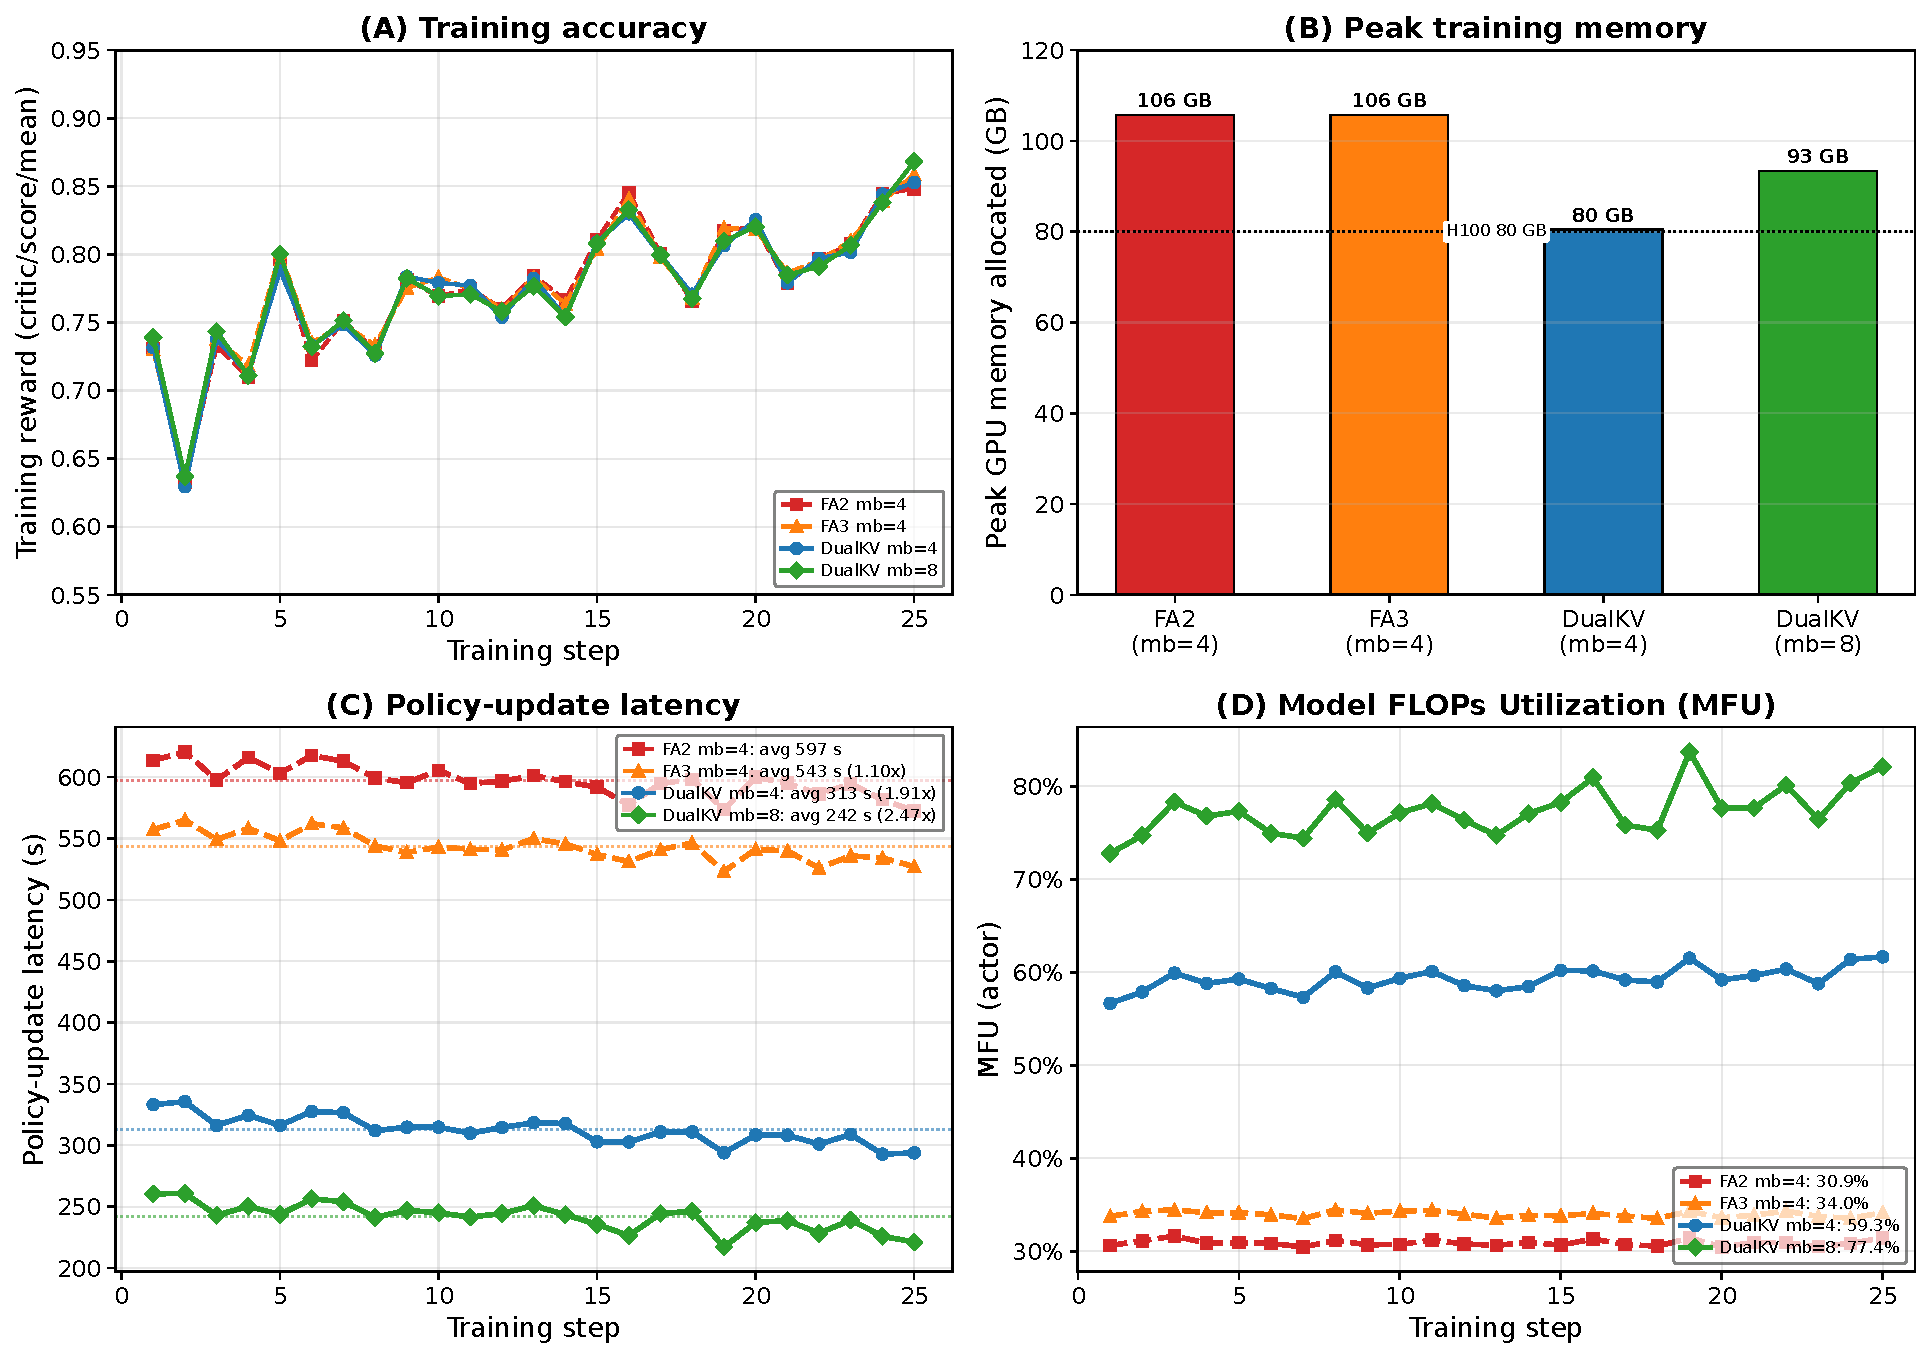
\includegraphics[width=\textwidth]{figures/dapo_longreason_comparison.pdf}
\caption{DAPO training on LongReason (Qwen3-8B, 8$\times$H100). \textbf{(A)}~All four configurations track identical reward curves, confirming no convergence degradation. \textbf{(B)}~Peak memory: FA2/FA3 exceed the H100 80\,GB physical limit (${\sim}106$\,GB allocated), while DualKV mb=4 fits at ${\sim}80$\,GB. \textbf{(C)}~Policy-update latency: DualKV mb=8 achieves $2.47\times$ speedup over FA2. \textbf{(D)}~MFU rises from $31\%$ (FA2) to $77\%$ (DualKV mb=8).}
\label{fig:dapo-longreason-comparison}
\end{figure}

\subsection{Context-Length Scaling Sweep (Llama-3.1-8B)}
\label{app:context-sweep}

To validate that DualKV's benefits generalize beyond Qwen and to empirically characterize memory scaling, we conduct a context-length sweep on Llama-3.1-8B-Instruct~\citep{dubey2024llama3} across prompt lengths $P \in \{8\text{K}, 16\text{K}, 32\text{K}, 48\text{K}, 64\text{K}, 96\text{K}\}$ and micro-batch sizes $\text{mb} \in \{4, 8, 16\}$.

\paragraph{Setup.} Hardware: 2$\times$\texttt{p5.48xlarge} (16$\times$H100-80GB). GRPO with $N{=}32$, $R_{\max}{=}2048$, \texttt{train\_batch\_size}${=}128$, vLLM rollout (TP${=}2$), DualKV + FusedLinearForPPO enabled, \texttt{gpu\_memory\_utilization}${=}0.4$.

\paragraph{Memory scaling law.} Figure~\ref{fig:memory-scaling-law} plots peak GPU memory (\texttt{max\_memory\_allocated}) against prompt length for all 18 configurations. DualKV's memory follows:
\begin{equation}
  \text{mem}_{\text{DualKV}} = \underbrace{M_0}_{\substack{\text{model + optim +}\\\text{framework}}} + \underbrace{c_P \cdot P}_{\substack{\text{prompt activations}\\\text{(paid once)}}} + \underbrace{c_{\text{mb}R} \cdot \text{mb} \cdot R}_{\substack{\text{response activations}\\\text{(scales with mb)}}}
  \label{eq:mem-scaling}
\end{equation}
where the coefficients are estimated by least-squares regression across all 18 data points ($6$ prompt lengths $\times$ $3$ micro-batch sizes): $M_0 \approx 41.1$\,GB, $c_P \approx 0.475$\,GB/Ktoken, $c_{\text{mb}R} \approx 0.122$\,GB/Ktoken ($r^2 = 0.989$). The asymmetry $c_P \gg c_{\text{mb}R}$ arises because prompt tokens incur higher per-token activation cost under gradient checkpointing: block-boundary activations are retained for all $P$ positions across all layers, and the context self-attention backward (Call~1) saves \texttt{softmax\_lse} of size $O(P \times H)$. Response tokens in Call~2 attend only to their own shorter decoded subsequence, requiring less stored state. The key insight is structural: the prompt term $c_P \cdot P$ does not multiply by mb --- DualKV processes the shared prompt once regardless of how many responses are in the micro-batch. Under standard FA2 packing, each of the mb sequences carries its own full copy of the prompt, so memory scales as:
\begin{equation}
  \text{mem}_{\text{FA2}} = \underbrace{M_0}_{\text{same}} + \underbrace{c_P \cdot \text{mb} \cdot (P + R)}_{\text{prompt replicated mb times}}
  \label{eq:mem-scaling-fa2}
\end{equation}
making memory \emph{linear in mb}. FA2 values in Figure~\ref{fig:memory-scaling-law} are projections from Eq.~\ref{eq:mem-scaling-fa2} (using the same fitted $M_0$ and $c_P$) rather than measurements, because FA2 triggers CUDA OOM at these context lengths --- the standard $\text{mb} \times (P + R)$ packing exceeds the H100's 80\,GB HBM for most configurations in this sweep.

\paragraph{Practical implication.} When $P \gg \text{mb} \cdot R$ (the long-prompt regime common in agentic and reasoning tasks), memory is dominated by the prompt term and becomes effectively independent of micro-batch size. Practitioners can freely increase mb to maximize GPU utilization without memory penalty: at $P{=}96\text{K}$, increasing mb from 4 to 16 adds only ${\sim}4$\,GB ($<5\%$), whereas FA2 would require $225 \to 775$\,GB --- nearly $10\times$ the physical capacity of an H100.

\begin{figure}[ht]
\centering
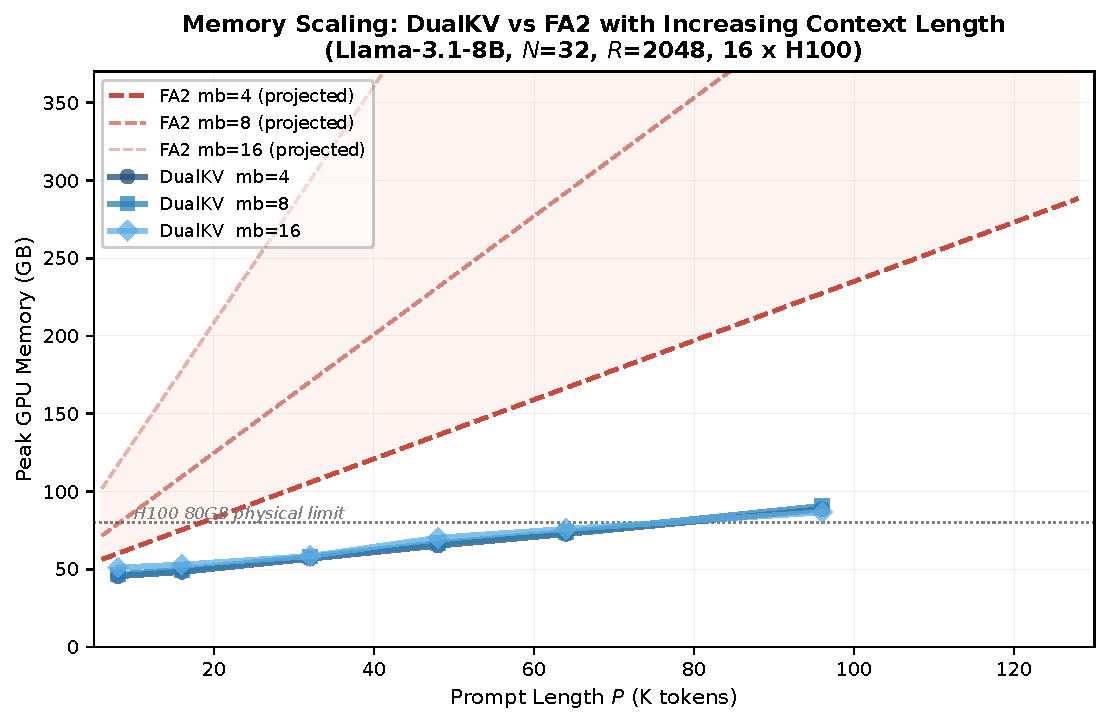
\includegraphics[width=0.85\textwidth]{figures/memory_scaling_law.pdf}
\caption{Memory scaling law: DualKV (measured, solid) vs.\ FA2 (projected, dashed). Llama-3.1-8B, $N{=}32$, $R{=}2048$, 16$\times$H100. DualKV's three micro-batch curves cluster tightly ($\text{mem} \propto P + \text{mb} \cdot R$), while FA2's diverge ($\text{mem} \propto \text{mb} \cdot (P+R)$). FA2 curves are projected from the fitted model since FA2 OOMs at these configurations.}
\label{fig:memory-scaling-law}
\end{figure}

\subsection{Comparison with Prefix Grouper: Single-Layer Benchmark}
\label{app:prefix-grouper-comparison}

To empirically validate DualKV's advantage over framework-level prefix sharing, we benchmark against Prefix Grouper~\citep{liu2025prefixgrouper} on a single Qwen3-8B decoder layer (forward + backward) on one H100-80GB GPU. Prefix Grouper decomposes attention into prefix self-attention and suffix cross-attention (2$\times$ FA2 calls), but operates on \emph{padded} 2D tensors: all $N$ sequences are padded to the longest response length and the full padded tensor passes through QKV projections, output projection, LayerNorm, and MLP. We give Prefix Grouper the best possible backend (padded \texttt{flash\_attn\_func}, not the default HuggingFace wrapper) and compare against both standard FA2 varlen (the baseline) and DualKV.

\paragraph{Setup.} Qwen3-8B dimensions ($H{=}32$, $H_k{=}8$, $d{=}128$), bf16, response lengths $R \sim U(131, 2048)$. We sweep prompt lengths $P \in \{5059, 8192, 16384, 32768, 65536, 131072\}$ and micro-batch sizes $\text{mb} \in \{1, 2, 4, 8, 16, 32\}$. Timing: 2 warmup + 5 measured iterations. Correctness verified via \texttt{torch.allclose} against FA2 at smaller configs (both DualKV and PG pass; PG has zero error since it uses FA2 internally).

\begin{table}[ht]
\centering
\small
\caption{Single-layer forward+backward: DualKV vs.\ Prefix Grouper (PG) vs.\ FA2. Time in ms, memory in GB. ``DK/FA2'' and ``DK/PG'' are DualKV's speedup ratios. OOM = out of memory on H100-80GB.}
\label{tab:prefix-grouper-comparison}
\setlength{\tabcolsep}{3.5pt}
\begin{tabular}{@{}rr|rrr|rr|rr@{}}
\toprule
& & \multicolumn{3}{c|}{\textbf{Time (ms)}} & \multicolumn{2}{c|}{\textbf{DualKV Speedup}} & \multicolumn{2}{c}{\textbf{Peak Memory (GB)}} \\
$P$ & mb & FA2 & DualKV & PG & vs FA2 & vs PG & DualKV & PG \\
\midrule
5K   & 4  & 93.2   & \textbf{36.6}  & 72.5   & 2.55$\times$ & 1.98$\times$ & \textbf{4.0}  & 9.0 \\
5K   & 8  & 153.3  & \textbf{61.4}  & 156.9  & 2.50$\times$ & 2.55$\times$ & \textbf{5.5}  & 18.1 \\
5K   & 16 & 338.9  & \textbf{110.4} & 314.2  & 3.07$\times$ & 2.85$\times$ & \textbf{9.0}  & 35.4 \\
5K   & 32 & 597.2  & \textbf{179.9} & 626.3  & 3.32$\times$ & 3.48$\times$ & \textbf{13.7} & 69.8 \\
\midrule
8K   & 4  & 148.9  & \textbf{57.2}  & 124.3  & 2.60$\times$ & 2.17$\times$ & \textbf{4.9}  & 12.8 \\
8K   & 8  & 245.4  & \textbf{70.3}  & 232.1  & 3.49$\times$ & 3.30$\times$ & \textbf{6.5}  & 25.8 \\
8K   & 16 & 549.2  & \textbf{128.2} & 465.4  & 4.28$\times$ & 3.63$\times$ & \textbf{9.9}  & 50.7 \\
8K   & 32 & \multicolumn{1}{c}{OOM} & \textbf{184.2} & \multicolumn{1}{c|}{OOM} & $\infty$ & $\infty$ & \textbf{14.6} & --- \\
\midrule
16K  & 4  & 329.9  & \textbf{108.9} & 245.7  & 3.03$\times$ & 2.26$\times$ & \textbf{7.5}  & 22.9 \\
16K  & 8  & 553.0  & \textbf{125.4} & 434.9  & 4.41$\times$ & 3.47$\times$ & \textbf{9.0}  & 45.9 \\
16K  & 16 & \multicolumn{1}{c}{OOM} & \textbf{205.8} & \multicolumn{1}{c|}{OOM} & $\infty$ & $\infty$ & \textbf{12.5} & --- \\
\midrule
32K  & 2  & 408.0  & \textbf{220.3} & 308.1  & 1.85$\times$ & 1.40$\times$ & \textbf{11.8} & 22.1 \\
32K  & 4  & 810.2  & \textbf{246.4} & 513.6  & 3.29$\times$ & 2.08$\times$ & \textbf{12.5} & 43.0 \\
32K  & 8  & \multicolumn{1}{c}{OOM} & \textbf{266.8} & \multicolumn{1}{c|}{OOM} & $\infty$ & $\infty$ & \textbf{14.1} & --- \\
\midrule
65K  & 2  & 1173.5 & \textbf{614.1} & 773.3  & 1.91$\times$ & 1.26$\times$ & \textbf{21.9} & 42.3 \\
65K  & 4  & \multicolumn{1}{c}{OOM} & \textbf{653.9} & \multicolumn{1}{c|}{OOM} & $\infty$ & $\infty$ & \textbf{22.7} & --- \\
65K  & 16 & \multicolumn{1}{c}{OOM} & \textbf{892.6} & \multicolumn{1}{c|}{OOM} & $\infty$ & $\infty$ & \textbf{27.7} & --- \\
\midrule
131K & 8  & \multicolumn{1}{c}{OOM} & \textbf{2096.7} & \multicolumn{1}{c|}{OOM} & $\infty$ & $\infty$ & \textbf{44.5} & --- \\
131K & 32 & \multicolumn{1}{c}{OOM} & \textbf{2883.0} & \multicolumn{1}{c|}{OOM} & $\infty$ & $\infty$ & \textbf{52.6} & --- \\
\bottomrule
\end{tabular}
\end{table}


\textbf{PG $\approx$ FA2 in latency.} Prefix Grouper's attention optimization (avoiding redundant prefix-on-prefix QK$^\top$) is offset by the overhead of padding, KV expansion (\texttt{expand + contiguous}), and concatenation. Across all configs where both run, PG is within $\pm$20\% of FA2 --- sometimes slightly faster (attention savings dominate at large $P$), sometimes slightly slower (padding overhead dominates at large mb).

\textbf{DualKV is 2--4$\times$ faster than both.} The speedup comes from processing fewer tokens through \emph{every} operation in the layer. At the paper's primary config ($P{=}8\text{K}$, mb=8), DualKV processes 18K tokens vs.\ FA2's 75K and PG's 81K --- a $4.2\times$ reduction that translates directly to a $3.5\times$ wall-clock speedup.

\textbf{Memory gap is catastrophic for PG.} PG allocates a padded $[\text{mb}, P+R_{\max}, H]$ tensor, consuming $3$--$5\times$ the memory of DualKV's packed representation. At $P{=}8\text{K}$ mb=16, PG uses 50.7\,GB vs.\ DualKV's 9.9\,GB ($5.1\times$ reduction); at mb=32, PG OOMs while DualKV fits in 14.6\,GB.

\textbf{Scalability.} Of 54 total configurations tested (9 prompt lengths $\times$ 6 micro-batch sizes), DualKV runs 36 configs, while both FA2 and PG run only 21. Beyond $P{=}131\text{K}$, only DualKV can scale past mb=1 on a single H100.

\textbf{Root cause: PG only optimizes attention.} Attention accounts for ${\sim}30\%$ of a decoder layer's FLOPs; the remaining 70\% (QKV projections, output projection, MLP, norms) still operates on the full padded tensor with $N$ duplicated prompt copies. DualKV eliminates redundancy across \emph{all} operations by packing the prompt once in a varlen representation.

%----------------------------------------------------------------------
\section{Additional Experimental Figures}
\label{app:additional-figures}
%----------------------------------------------------------------------

\begin{figure}[ht]
\centering
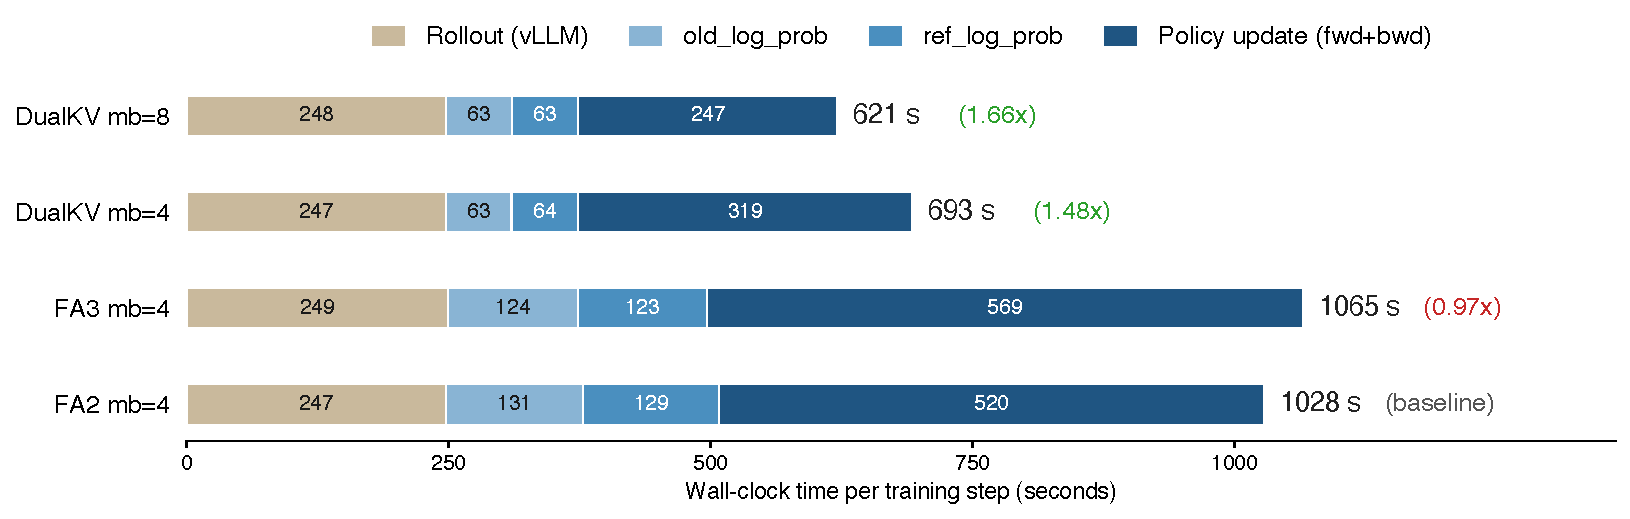
\includegraphics[width=1.05\textwidth]{figures/longreason_step_breakdown.pdf}
\caption{Per-phase breakdown of an average GRPO training step on LongReason (Section~\ref{sec:e2e-longreason}). DualKV compresses the three training-side phases (\texttt{old\_log\_prob}, \texttt{ref\_log\_prob}, \texttt{policy update}) by ${\sim}2\times$ each; rollout latency is identical across all four configs. \textbf{(i)} the policy-update slice shrinks from $520$\,s (FA2, FA3) to $247$\,s ($2.1\times$ over FA2); \textbf{(ii)} the rollout slice is invariant (${\sim}247$\,s across all four configs); \textbf{(iii)} rollout's share of step time grows from $23\%$ (FA2 mb=4) to $40\%$ (DualKV mb=8) --- DualKV shifts the bottleneck from the policy update to rollout generation.}
\label{fig:longreason-step-breakdown}
\end{figure}

\begin{figure}[ht]
\centering
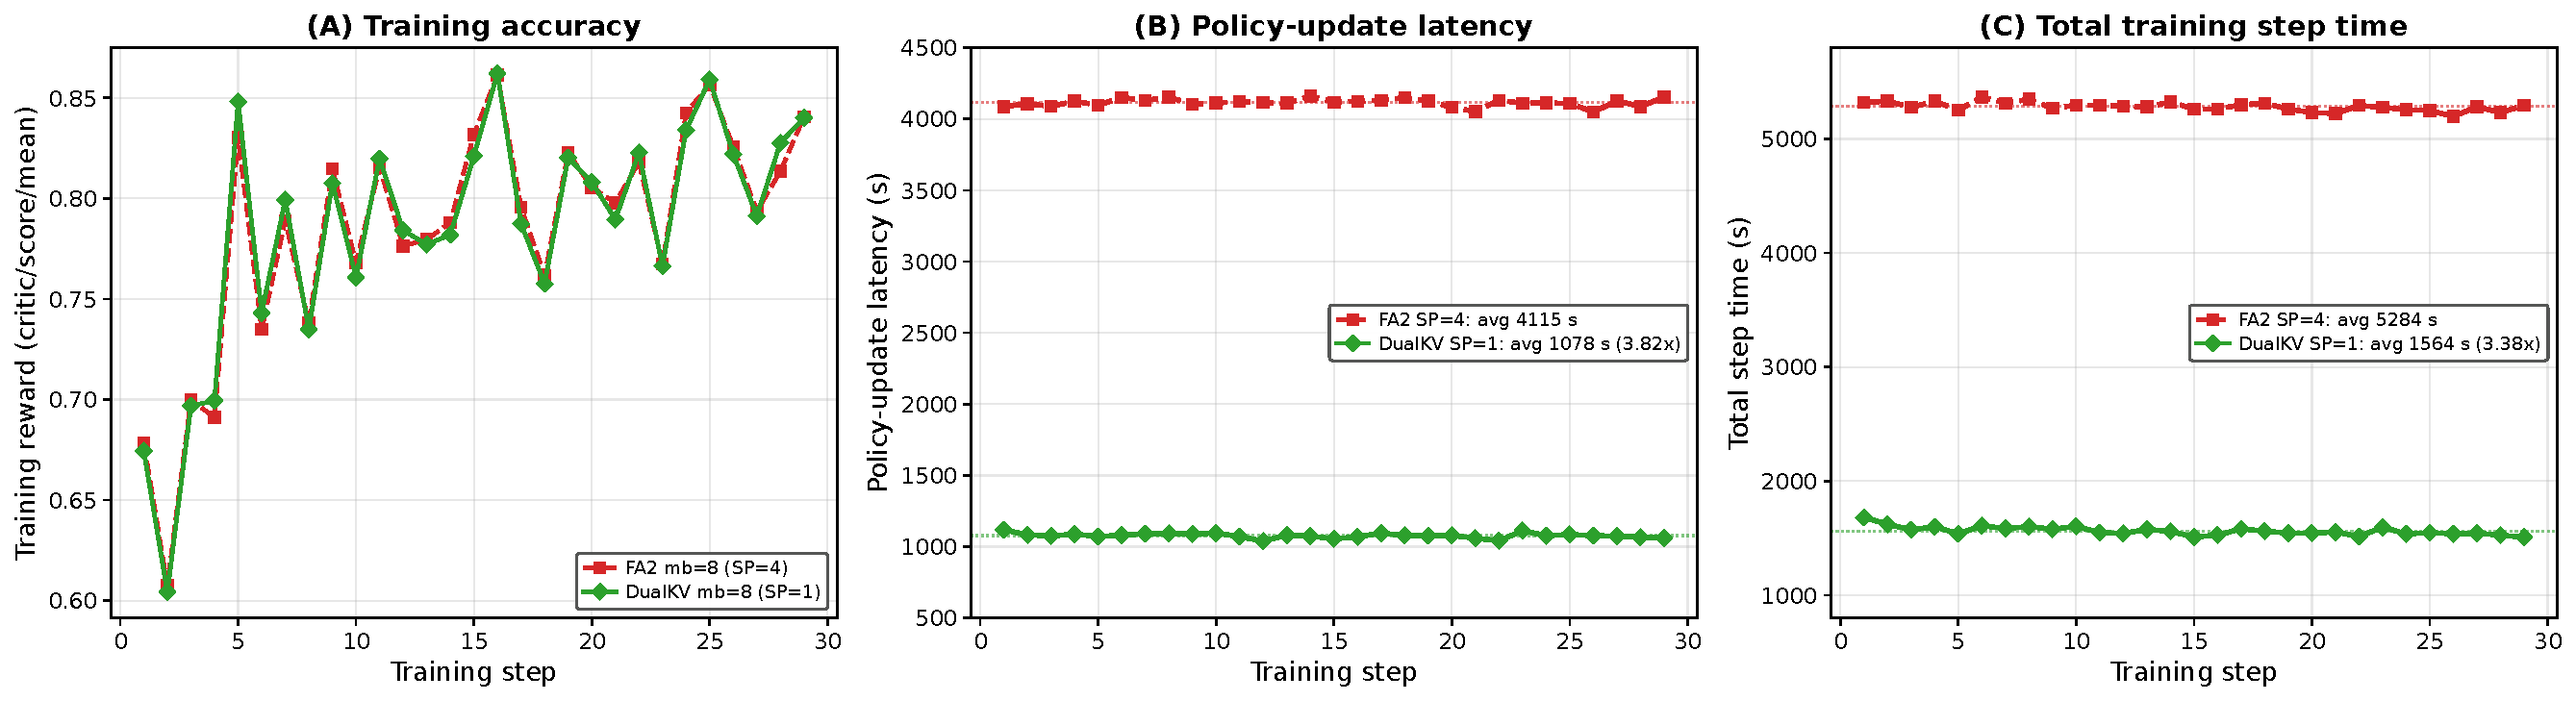
\includegraphics[width=1.05\textwidth]{figures/moe_multinode_comparison.pdf}
\caption{Multi-node MoE GRPO training on LongReason (Section~\ref{sec:e2e-moe-multinode}; Qwen3-30B-A3B, 16$\times$H100, 2 nodes), comparing DualKV mb=8 SP=1 against FA2 mb=8 SP=4 over the common 1--29-step window. \textbf{(A)} Per-step training reward --- both configs track closely. \textbf{(B)} Per-step policy-update latency --- DualKV averages 1078\,s vs FA2's 4115\,s ($3.82\times$). \textbf{(C)} Per-step total training step time --- DualKV averages 1564\,s vs FA2's 5284\,s ($3.38\times$).}
\label{fig:moe-multinode}
\end{figure}

\begin{figure}[ht]
\centering
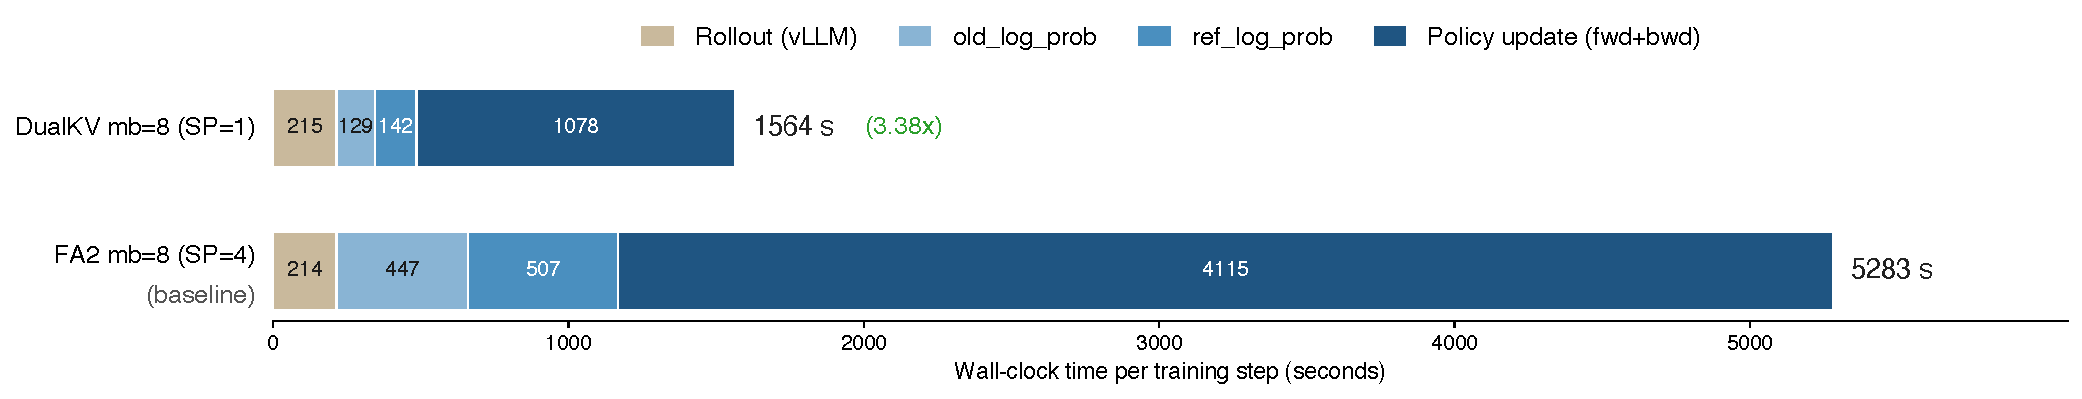
\includegraphics[width=1.05\textwidth]{figures/moe_multinode_step_breakdown.pdf}
\caption{Per-phase breakdown of an average GRPO training step for the multi-node MoE experiment (Section~\ref{sec:e2e-moe-multinode}). DualKV compresses the three training-side phases by $3.4$--$3.6\times$ each; rollout latency is identical across both configs. The FA2 bar uses 4-way Ulysses SP --- the smallest SP that avoids OOM at this scale --- while DualKV runs at SP=1.}
\label{fig:moe-multinode-breakdown}
\end{figure}

%----------------------------------------------------------------------
\section{DualKV Kernel Algorithms}
\label{app:kernel-algorithms}
%----------------------------------------------------------------------

This appendix gives full pseudocode for the DualKV forward and backward kernels (referenced from Sections~\ref{sec:kernel-forward}--\ref{sec:kernel-backward}). The listings elide K/V parallels: gradients, loads, and writes for $V$ mirror those for $K$ and are omitted for brevity.

\begin{algorithm}[H]
\small
\caption{DualKV forward kernel (one thread block, assigned $(m, b, h)$ = query-row block, batch, head)}
\label{alg:dualkv-forward}
\begin{algorithmic}[1]
\Require $Q_m$ for batch $b$, head $h$; shared $K_c, V_c \in \mathbb{R}^{P \times H_k \times d}$; per-sequence $K_d^{(b)}, V_d^{(b)} \in \mathbb{R}^{R_b \times H_k \times d}$; tile size $B_N$; $P$ (= \texttt{context\_seqlen})
\State $n_{\text{ctx}} \gets \lceil P / B_N \rceil$
\State $n_{\text{dec}} \gets \lceil R_b / B_N \rceil$
\State $n_{\max} \gets n_{\text{ctx}} + n_{\text{dec}}$
\State Apply causal pruning: reduce $n_{\max}$ so no tile exceeds the causal horizon of $Q_m$
\State Init $m_i \gets -\infty$,\; $\ell_i \gets 0$,\; $\mathbf{o}_i \gets 0$ \Comment{online-softmax state per row in $Q_m$}
\For{$n = n_{\max}{-}1$ down to $0$} \Comment{iterate K-tiles in reverse (FA2 convention)}
    \If{$n < n_{\text{ctx}}$} \Comment{context tile: shared buffer}
        \State $K_n, V_n \gets K_c[n B_N : n B_N + B_N], V_c[\ldots]$
        \State $j_{\text{base}} \gets n \cdot B_N$ \Comment{logical K position}
    \Else \Comment{decoded tile: per-sequence buffer}
        \State $K_n, V_n \gets K_d^{(b)}[(n{-}n_{\text{ctx}}) B_N : \ldots]$
        \State $j_{\text{base}} \gets P + (n - n_{\text{ctx}}) \cdot B_N$
    \EndIf
    \State Mask out-of-bounds lanes (partial tile at last context / last decoded tile)
    \State $S \gets Q_m K_n^\top / \sqrt{d}$
    \State Apply causal mask using $j_{\text{base}}$ (logical K position) vs.\ $Q_m$'s logical row position
    \State $m_i^{\text{new}} \gets \max(m_i,\; \text{rowmax}(S))$
    \State $P \gets \exp(S - m_i^{\text{new}})$
    \State $\alpha \gets e^{m_i - m_i^{\text{new}}}$ \Comment{online-softmax rescale factor}
    \State $\ell_i \gets \alpha \, \ell_i + \text{rowsum}(P)$
    \State $\mathbf{o}_i \gets \alpha \, \mathbf{o}_i + P \cdot V_n$
    \State $m_i \gets m_i^{\text{new}}$
\EndFor
\State $\mathbf{o}_i \gets \mathbf{o}_i / \ell_i$ \Comment{epilogue: normalize}
\State Write $\mathbf{o}_i$ to $o[m]$
\State Save $L = m_i + \log \ell_i$ to \texttt{softmax\_lse}[m] \Comment{used by backward}
\end{algorithmic}
\end{algorithm}

The backward main kernel (Algorithm~\ref{alg:dualkv-backward}) and the post-kernel context-gradient cast (Algorithm~\ref{alg:dualkv-bwd-convert}) are in Section~\ref{sec:kernel-backward}.

%----------------------------------------------------------------------
\section{Kernel Interface: Python Signature and Tensor Shapes}
\label{app:kernel-interface}
%----------------------------------------------------------------------

This appendix gives the full Python signature of the DualKV kernel (referenced from Section~\ref{sec:kernel}) and the per-tensor shape contract.

\begin{lstlisting}[language=Python, caption=Signature of DualKV kernel interface \texttt{flash\_attn\_dualkv\_varlen\_func}]
out = flash_attn_dualkv_varlen_func(
    q,                      # (sum_Ri, H,   d)   decoded queries, packed varlen
    k_context, v_context,   # (P,      H_k, d)   shared context KV (single copy)
    k_decoded, v_decoded,   # (sum_Ri, H_k, d)   per-sequence decoded KV, packed varlen
    cu_seqlens_q,           # (N+1,)             varlen offsets into q, k_decoded, v_decoded
    cu_seqlens_k_decoded,   # (N+1,)             same offsets (context is shared)
    max_seqlen_q,           # int                max R_i
    context_seqlen,         # int = P            causal offset: decoded query at index r
                            #                      has logical position P + r
    max_seqlen_k_decoded,   # int                max R_i
    softmax_scale=None,     # float              defaults to 1/sqrt(d)
    causal=True,            # bool               training always sets True
)
\end{lstlisting}

The key contract is that $k_{\text{ctx}}$ and $v_{\text{ctx}}$ (\texttt{k\_context}, \texttt{v\_context} in the listing) are stored once (not replicated $N$ times), while $q$, $k_{\text{dec}}$, and $v_{\text{dec}}$ are varlen-packed over the $N$ decoded sequences. The kernel is implemented as a PyTorch \texttt{torch.autograd.Function}. Internally, the forward also computes a per-query softmax log-sum-exp tensor \texttt{softmax\_lse} of shape $(H, \sum_i R_i)$ that is saved onto the autograd context for the backward pass (Section~\ref{sec:kernel-backward}); it is not part of the user-facing return value.

% \begin{table}[ht]
% \centering
% \small
% \caption{DualKV kernel tensor shapes. $H$ = query heads, $H_k$ = KV heads (GQA), $d$ = head dim.}
% \label{tab:dualkv-shapes}
% \begin{tabular}{@{}lll@{}}
% \toprule
% \textbf{Tensor} & \textbf{Shape} & \textbf{Storage} \\
% \midrule
% $q$                 & $(\sum_i R_i,\; H,\; d)$   & per-sequence, packed varlen \\
% $k_{\text{ctx}}, v_{\text{ctx}}$ & $(P,\; H_k,\; d)$ & shared across sequences \\
% $k_{\text{dec}}, v_{\text{dec}}$ & $(\sum_i R_i,\; H_k,\; d)$ & per-sequence, packed varlen \\
% output $o$          & $(\sum_i R_i,\; H,\; d)$   & per-sequence, packed varlen \\
% \bottomrule
% \end{tabular}
% \end{table}

%----------------------------------------------------------------------
\section{Comparison with Other Attention Variants}
\label{app:attention-comparison}
%----------------------------------------------------------------------

Readers familiar with attention-optimization literature may ask whether existing variants --- paged attention, prefix caching, bifurcated attention, sequence-parallel methods, or sparse/linear attention --- already address the shared-prompt redundancy we target. This appendix systematically positions DualKV against these variants along four capabilities relevant to RL policy-update training:

\begin{enumerate}
  \item \textbf{Shared-prompt KV dedup}: the method stores the shared prompt's $K, V$ once rather than $N$ times.
  \item \textbf{Shared-prompt compute dedup}: the method also processes the shared prompt through per-token operations (RMSNorm, QKV projection, RoPE, MLP, output projection) \emph{once} rather than $N$ times --- i.e., eliminates the $(N{-}1) \cdot P$ tokens of compute outside attention.
  \item \textbf{Training backward + autograd integration}: the method provides a differentiable backward pass, with gradients for all inputs compatible with PyTorch autograd (including gradient accumulation into the shared $K_c, V_c$ across the $N$ concurrent sequences).
  \item \textbf{Mathematically exact}: the method produces outputs identical to standard attention up to floating-point rounding, not an approximation.
\end{enumerate}

Table~\ref{tab:attention-comparison} summarizes the comparison. DualKV is the only variant that satisfies all four criteria simultaneously.

\begin{table}[ht]
\centering
\scriptsize
\setlength{\tabcolsep}{4pt}
\caption{Comparison of attention variants along four capabilities relevant to RL training. $\checkmark$ = satisfies; $\times$ = does not. DualKV is the only variant that is $\checkmark$ on all four.}
\label{tab:attention-comparison}
\begin{tabular}{@{}l c c c c@{}}
\toprule
\textbf{Variant} & \textbf{KV dedup} & \textbf{Compute dedup} & \textbf{Training bwd} & \textbf{Exact} \\
\midrule
FlashAttention-2/3~\citep{dao2023flashattention2,shah2024flashattention3} & $\times$ & $\times$ & $\checkmark$ & $\checkmark$ \\
Paged Attention~\citep{kwon2023vllm}              & storage only       & $\times$ & $\times$  & $\checkmark$ \\
SGLang RadixAttention~\citep{zheng2023sglang}     & storage only       & $\times$ & $\times$  & $\checkmark$ \\
Bifurcated Attention~\citep{athiwaratkun2024bifurcated} & attn.\ only & $\times$ & $\times$  & $\checkmark$ \\
Ring Attention~\citep{liu2023ringattention}        & $\times$           & $\times$ & $\checkmark$       & $\checkmark$ \\
Ulysses SP~\citep{jacobs2023ulysses}              & $\times$           & $\times$ & $\checkmark$       & $\checkmark$ \\
Linear / sparse attention                          & $\times$           & $\times$ & $\checkmark$       & $\times$ (approx.) \\
KV-cache compression (H2O, SnapKV, etc.)           & $\times$           & $\times$ & $\times$ & $\times$ (lossy) \\
\midrule
\textbf{DualKV (ours)}                             & $\checkmark$       & $\checkmark$ & $\checkmark$   & $\checkmark$ \\
\bottomrule
\end{tabular}
\end{table}

\paragraph{Inference-only variants (paged, RadixAttention, bifurcated).} These methods share the shared-prompt KV at \emph{storage} level (via block tables or memory-layout tricks) during inference. None defines a backward pass for training. Naively invoking a paged or bifurcated kernel in a training loop would fail because (i) PyTorch autograd cannot differentiate through block-table pointer indirection --- the shared KV must be a proper tensor with a computation graph; (ii) with $N$ concurrent sequences backward-propagating into the \emph{same} $K_c, V_c$, the gradient accumulation requires race-free concurrent writes with precision preservation (DualKV's fp32 atomic accumulation, Section~\ref{sec:kernel-backward}); and (iii) they address attention only, leaving the $(N{-}1) \cdot P$ per-token cost in MLP, norms, and projections unaffected.

\paragraph{Sequence-parallel variants (Ring, Ulysses).} These are orthogonal techniques for long-sequence training: they shard a \emph{single} long sequence across multiple ranks via collective communication. They do not deduplicate the \emph{shared prompt across multiple sequences} --- that is a different axis of redundancy. DualKV composes with sequence parallelism; combining the two is an interesting future direction.

\paragraph{Approximate variants (linear, sparse, compressed).} These trade accuracy for efficiency by replacing attention with $O(S)$ approximations or by pruning KV entries. They violate DualKV's ``mathematically equivalent to standard attention'' guarantee, and are orthogonal to shared-prompt dedup --- they can be applied per-sequence independently of whether sequences share a prompt.

\paragraph{Summary.} DualKV is the first attention variant to jointly provide (1) shared-prompt KV dedup, (2) shared-prompt compute dedup through the full transformer layer, (3) a mathematically exact training backward with gradient accumulation into the shared $K_c, V_c$, and (4) autograd-compatible integration with PyTorch. No existing technique can be dropped into a RL policy-update pipeline to replicate DualKV's savings.

% %%%%%%%%%%%%%%%%%%%%%%%%%%%%%%%%%%%%%%%%%%%%%%%%%%%%%%%%%%%%
% \newpage
% \input{checklist.tex}

\end{document}
